% The PyCBC Live ranking statistic in O3 was a very simple Phase-time-amplitude
% To improve the ranking statistic in O4 we have included measurements of the noise background and template dependent ranking
% Including these template fits in Live has a demonstrated sensitivity improvement of 10% for 0.5 IFAR and 39% for 1 IFAR in an `offline' pseudo live injected set test of the PyCBC Live search.
% These fits are generated every week based on the previous week of triggers to be used for the next week of data searching
% Currently gearing up for MDC testing with intentions to be used ASAP


\section{Updated Ranking Statistic}

\subsection{What does the Ranking Statistic do?}

\subsection{Previous Coincident Detector Ranking Statistic}
% The PyCBC Live ranking statistic in O3 was a very simple Phase-time-amplitude

The PyCBC Live search in the third observing run assigned ranking statistic values to events based on single detector new SNR values, calculated using matched filter SNR and two signal consistency tests, and a coincident detector phase-time-amplitude consistency. The single detector ranking statistic used was \verb|newsnr_sgveto|, re-weighting matched filter SNR by the Allen-$\chi^{2}$~(cite Allen) and sine-gaussian $\chi^{2}$ values-(cite sine-gaussian). The coincident detector ranking statistic was \verb|PhaseTD|~(cite phasetd), comparing ratios of SNR and amplitudes alongside checking phase and time differences between triggers in online detectors and a measure of detector sensitivity at the time of the trigger.

\subsection{Template Dependent Noise Background Fitting}
% To improve the ranking statistic in O4 we have included measurements of the noise background and template dependent ranking
The ranking statistic assumes a Gaussian, stationary noise model for every template in our template bank. In the PyCBC Offline search we empirically measure the noise SNR distributions of each template instead of using the Gaussian noise model, then the triggers are ranked by how frequently its associated template triggers with high SNR in noise.

To do this we create a histogram of count vs SNR for each template and fit an exponential fitting factor to the slope of the distribution, we also count the number of triggers found above a pre-defined threshold SNR (currently $\rho_{thresh} = 6.0$). Then we calculate a noise rate for each template using the single detector new SNR values and these parameters (exponential fitting factor, $\alpha$, and rate above threshold, $\mu$).
%
equation
%
%

\begin{figure}
  \centering
  \begin{minipage}[t]{1.0\linewidth}
  
    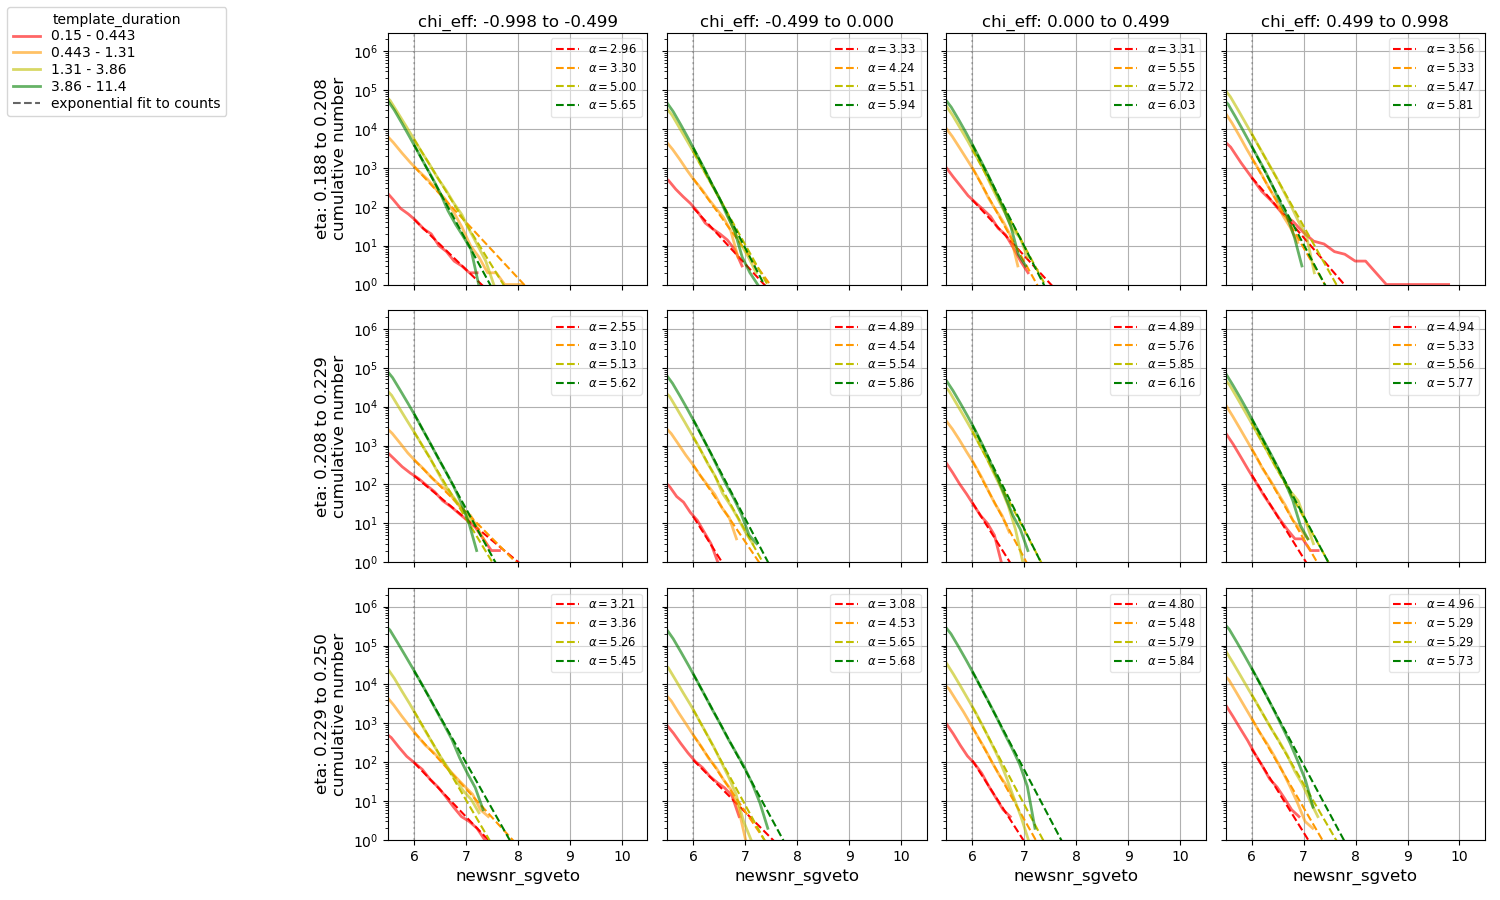
\includegraphics[width=1.0\textwidth]{images/pycbclive/H1-template_fits.png}
    \label{fig:pycbclive-H1-fits}
  
    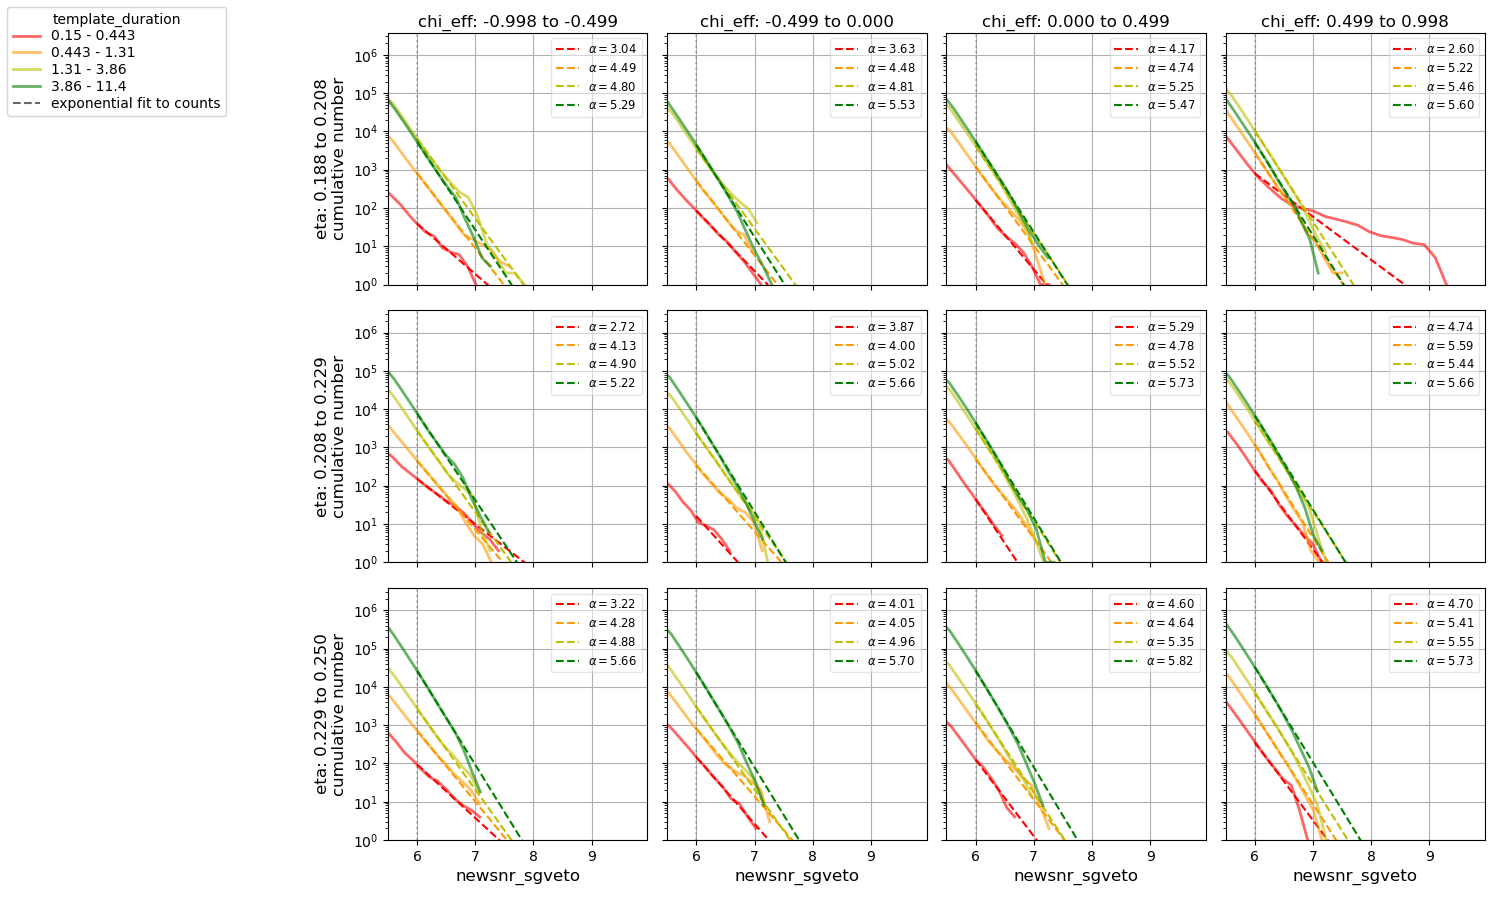
\includegraphics[width=1.0\linewidth]{images/pycbclive/L1-template_fits.png}
    \label{fig:pycbclive-L1-fits}

  \end{minipage}
  \caption{The noise distributions for 12 discrete bins in the $\chi_{eff}$ and $\eta$ parameter space, with cumulative number on the vertical axis and $\rho_{new}$ on the horizontal axis. Each bin then has four discrete template duration bins plotted on top, alongside the exponential fit factor for each template bin. The top plot represents the triggers from the H1 detector and the bottom plot the L1 detector triggers.}
  \label{fig:pycbclive-template-fits}
\end{figure}
%

\subsection{Ranking Statistic Formulation}
The previous ranking statistic calculated the ranking statistic like this:
%
equation
%
whereas in our new statistic we are using this formula,
%
equation.
%
This new formulation takes the noise rate and signal rates into account differently and as you can see, the new statistic includes two new components that were previously not seen in the old statistic
%
1 and 2.
%

This new formulation takes equal contribution from noise and signal rate.

\subsection{Sensitivity Improvements}
% Including these template fits in Live has a demonstrated sensitivity improvement of 10% for 0.5 IFAR and 39% for 1 IFAR in an `offline' pseudo live injected set test of the PyCBC Live search.
To estimate sensitivity improvements in the Live search from including the template fits we have performed an injection set test in `offline' with a pseudo-Live search which uses the PyCBC Live search script but the data is all pregenerated and therefore not running in real time but at the limits of computational processing as to how quickly it will search through all the data.

This offline test was performed on a injection set of BBH only signals and a the BBH focussed template bank from the third observing run. An MDC test using the full PyCBC Live template bank is currently being performed (who knows when).

To measure sensitivity improvements of this injection set we ran this search using the old statistic and our new statistic and compared the IFAR found for each injection at discrete IFAR thresholds. The IFAR of each injection found by both search can be seen in figure~below.
%
IFAR vs IFAR plot
sensitivity plot
%
We expect to see an increase in the number of injections found with an IFAR greater than the threshold when using the new statistic. The sensitivity improvement at different IFAR thresholds can be seen in figure~above2. Two commonly chosen IFAR thresholds are IFAR = 0.5 years, 1 year where we see a sensitivity increase of 10\% and 30\% respectively.

\subsection{Implementation in the Live Search}
% These fits are generated every week based on the previous week of triggers to be used for the next week of data searching
% Currently gearing up for MDC testing with intentions to be used ASAP
The PyCBC Offline searches through a week of data and creates the template fits after all triggers have been found. We are unable to do this in Live so we choose to use the previous week of triggers and assume they will still be representative of the next weeks noise distributions. In a case where the detectors have changed significantly the fit files can be regenerated or there will only  be a week of lag time on updating them.

The template fit files are created on the previous week of data and then loaded into the Live search and will be used for another week. We are currently preparing an MDC test of these changes with the hope of getting them into the PyCBC Live search on real gravitational wave data as soon as possible.







\section{\label{sec:pycbclive-sensitivity-improvements}Improvements in Sensitivity}

We measure improvement to the live search by performing injection set tests. The injection sets are made up of thousands of gravitational wave signals that are injected at a rate of approximately one every $100$ seconds. Initially we ran two `live' searches for gravitational waves, one with the old ranking statistic and one with the new ranking statistic which includes the additions of both PSD variation and template fitting.

The injection set used for this test is made up entirely of BBH signals to reduce the size of the template bank required~\cite{gwtc3}, there is a limit to the amount of memory a user can request for this pseudo-live search and therefore we couldn't initially test these changes on the full live template bank. The template bank of $15,436$ templates covers the BBH signal parameter space and is described in this paper~\cite{gwtc3}, this is far fewer than the full template bank being used by the PyCBC Live full bandwidth search which has over $730,000$ templates.

We used two weeks of O3b gravitational wave data, from 06 January 2020 23:59:42 - 20 January 2020 23:59:42, where the first week was used to generate the template fit statistic files and the second week was used to test the sensitivity improvements of the new additions to the ranking statistic. The injected gravitational wave data was created before the live searches were run and both searches were run on exactly the same data. The first week contained no gravitational wave injections and according to GraceDB, no real gravitational wave signals, the second week is where we injected the gravitational wave injection set.

A real live search will wait for new data before moving forward by eight seconds, we emulate the live search but all the data is readily available (in the form of pregenerated data) and it was processed as fast as the computational resources will allow. Therefore, running the live search over a week of data does not have to take a whole week and can take as little as 24 hours, decreasing with more computational resources assigned to it.

Once both searches have completed we can count the number of injections found by both searches. With the same template bank and data both searches should find the exact same triggers before any ranking is done, therefore we might expect to see the same number of injections but with different significance. In reality computing isn't always perfect and the number of injections found can be different between these two searches. We can associate each injection found by the searches with it's corresponding injection in our injection file and directly compare the injections found by both search, as we want to identify the significance change caused by the introduction of the new components to the ranking statistic.

We produce a list of injections seen by both searches and directly compare the false alarm rate (or inverse false alarm rate, IFAR) of each injection to see if there has been an improvement. We hope to see an decrease in the FAR (a lower false alarm rate) and therefore an increase in the IFAR. Each of these events is a real gravitational wave signal so we hope to see every single injection with a large IFAR value to indicate that the changes to the ranking statistic has improved the sensitivity of the search. Figure~\ref{fig:pycbclive-ifar-ifar-psdvar-4s} displays the IFAR for each injection with the new statistic (both PSD variation and template fits) on the y-axis and the x-axis the old statistic IFAR values.
%
\begin{figure}
  \centering
  \begin{minipage}[t]{1.0\linewidth}
  
    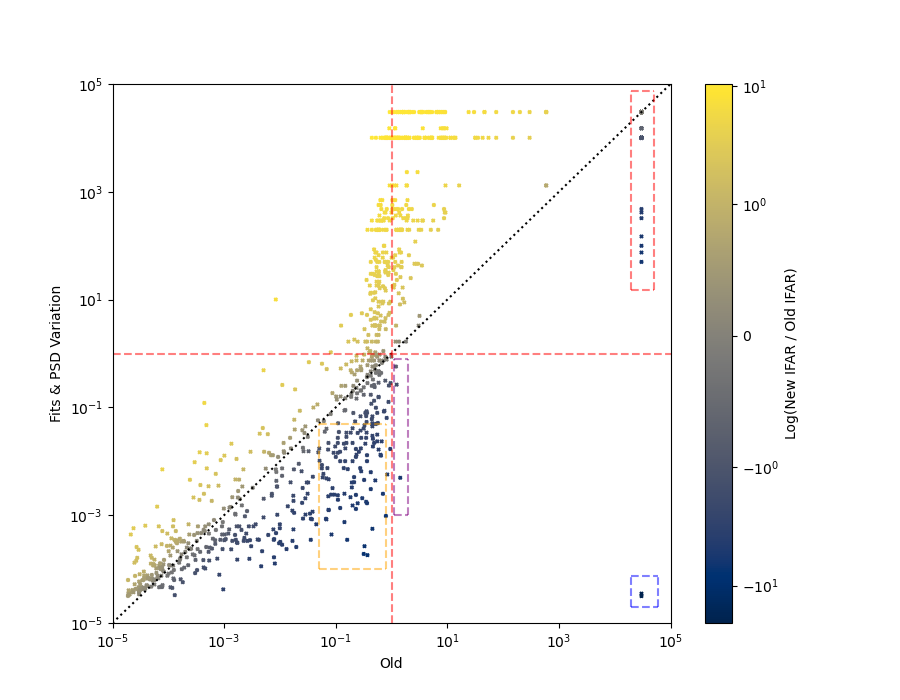
\includegraphics[width=0.9\textwidth]{images/pycbclive/psdvar_4s_ifar_vs_ifar_regions.png}
    \caption{Each point represents an injection in the injection set. The y values are the IFAR recorded from the new Template Fits and PSD Variation search, and the x value is the IFAR value when found with the old statistic. The colour bar represents the log difference in the IFAR of the two searches. The dashed line at $y=x$ represents an injection having the same IFAR in both the new and the old search. The vertical and horizontal lines represent an IFAR threshold of $1$ year, above which an injection might be considered real.}
    \label{fig:pycbclive-ifar-ifar-psdvar-4s}
  
    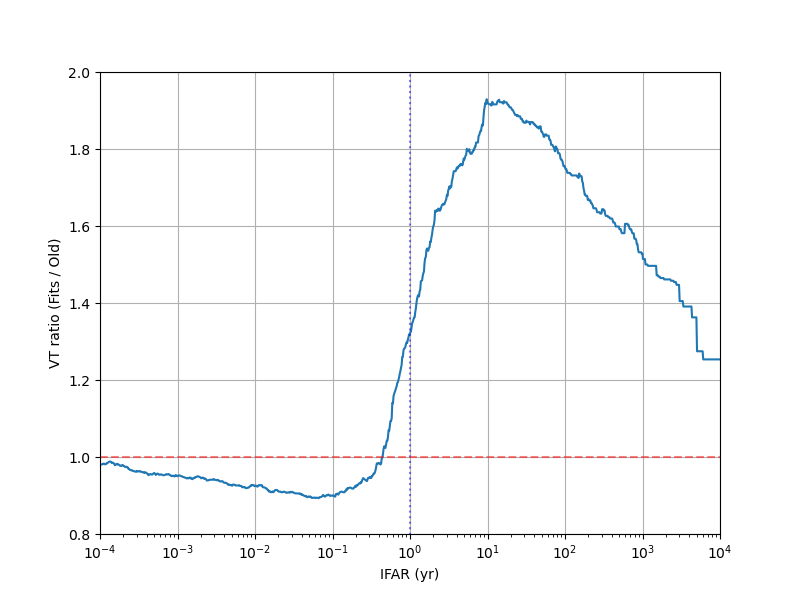
\includegraphics[width=0.9\textwidth]{images/pycbclive/ratio.png}
    \caption{The VT ratio between the new search and the old search. Calculated by sampling counting the number of injections found in both searches with an IFAR above the x value and dividing the number in the new search by the number from the old search.}
    \label{fig:pycbclive-psdvar-4s-sensitivity}

  \end{minipage}
\end{figure}
%
Within figure~\ref{fig:pycbclive-ifar-ifar-psdvar-4s} we have plotted a vertical and horizontal dotted line at an IFAR of 1 year to indicate a commonly chosen IFAR threshold above which an event would be considered 'real'. Therefore, this figure can be split into four quadrants: top-left, injections originally found below the IFAR threshold with the old statistic and now found above it with the new statistic; top-right, injections found in both searches; bottom-left, injections below the threshold in both searches; bottom-right, injections originally found above the IFAR threshold but now found below threshold with the new statistic. Another line has been plotted at y=x, injections above this line ($y > x$) have been found with a larger IFAR with the new statistics and injections below ($y < x$) have been found with a lower IFAR with the new statistic. We hope that every injection is found by the new statistic with a greater IFAR and therefore all injections will lie above the $y = x$ diagonal line.

To measure the sensitivity improvements of the new statistic we count the number of injections found with an IFAR over a certain value in both searches. If we do this for a range of IFAR values then we can build up an image of the sensitivity increase when using the new statistic. Figure~\ref{fig:pycbclive-psdvar-4s-sensitivity} shows this ratio of new statistic over old statistic.

The new statistic at an IFAR of 1 year can be seen to have found approximately 35\% more gravitational wave signals with an IFAR greater than 1 year. This is a large increase and demonstrates the benefit of adding the PSD variation and templates fits to the live search. Another commonly used threshold is $2 per year$ (IFAR$ = 0.5$) where we see a sensitivity increase of $10\%$.

We will investigate particular regions of the IFAR vs IFAR space, highlighted by dashed boxes in figure~\ref{fig:pycbclive-ifar-ifar-psdvar-4s}. These regions have been downranked by the new statistic and we want to understand why this has occurred and if any other changes can be made to the ranking statistic or if the search can be improved to avoid these injections being downranked.

\section{\label{pycbclive-ignoring-psdvar}Ignoring PSD Variation}

Figure~\ref{fig:pycbclive-ifar-ifar-psdvar-4s} shows a number of outlier injections which have been found with a much lower IFAR when found with the new statistic when compared to the old statistic,the bottom right region highlighted by a blue box. This is not desirable, especially when concerning the bottom-right quadrant where we initially observed the injection with a significance above threshold, we do not want to miss these with the new statistic.

The first avenue of exploration to identify the cause of the downranking in this region is with the new additions in the ranking statistic. These can be split into the inclusion of PSD variation and template fitting. We already had reservations using the PSD variation in live due to the nature of the live search and its ever adjusting PSD so we can remove the PSD variation contribution to the ranking statistic and check the IFARs of the injections with template fitting only. The IFAR vs IFAR figure for fitting only and the old statistic can be seen in figure~\ref{fig:pycbclive-ifar-ifar-fits-only-4s} and,
%
\begin{figure}
       \centering
    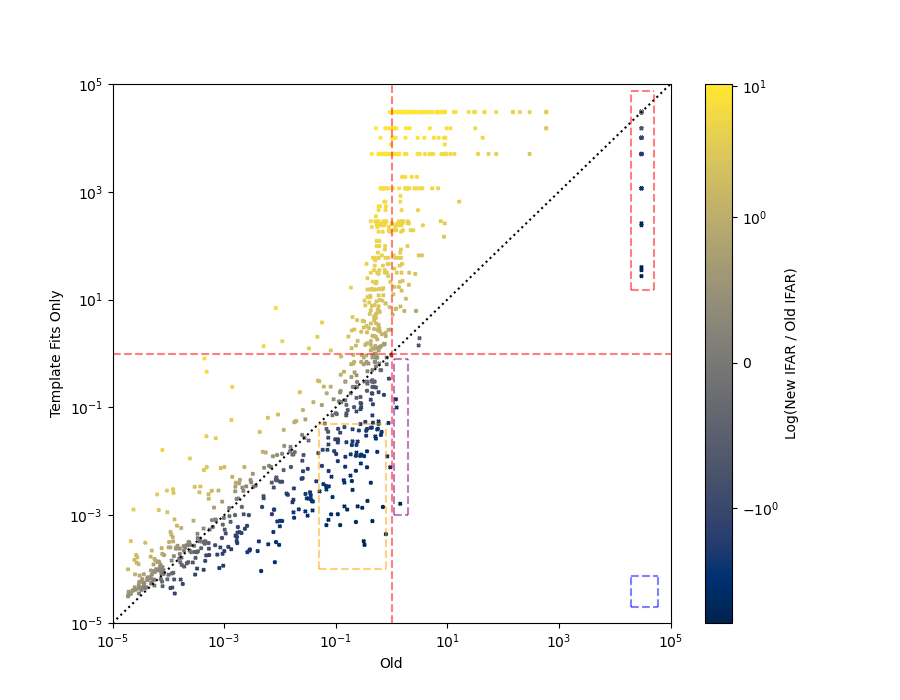
\includegraphics[width=1.2\textwidth]{images/pycbclive/fits_only_4s_ifar_vs_ifar_regions.png}
    \caption{}
    \label{fig:pycbclive-ifar-ifar-fits-only-4s}
\end{figure}
%
when compared to figure~\ref{fig:pycbclive-ifar-ifar-psdvar-4s} we can see the problematic injections in the bottom right corner of the figure have been removed. A direct comparison of the IFARs of the injections in the case of including only template fitting in the new statistic versus including both the PSD variation and the template fitting can be seen in figure~\ref{fig:pycbclive-ifar-ifar-fits-psdvar}. In this comparison, $550$ injections were found with a higher significance when \textbf{not} including PSD variation, $399$ were found with a higher IFAR when including PSD variation and $326$ were found with the same IFAR. This tells us that the PSD variation can help for some injections but it hinders the search more than it helps, especially when considering the injections in the top-left of figure~\ref{fig:pycbclive-ifar-ifar-fits-psdvar} which are losing a large amount of significance by including PSD variation.

We can produce the sensitivity plots to compare the template fitting only statistic against old statistic and the template fitting \& PSD variation against template fitting only searches.
%
\begin{figure}
       \centering
    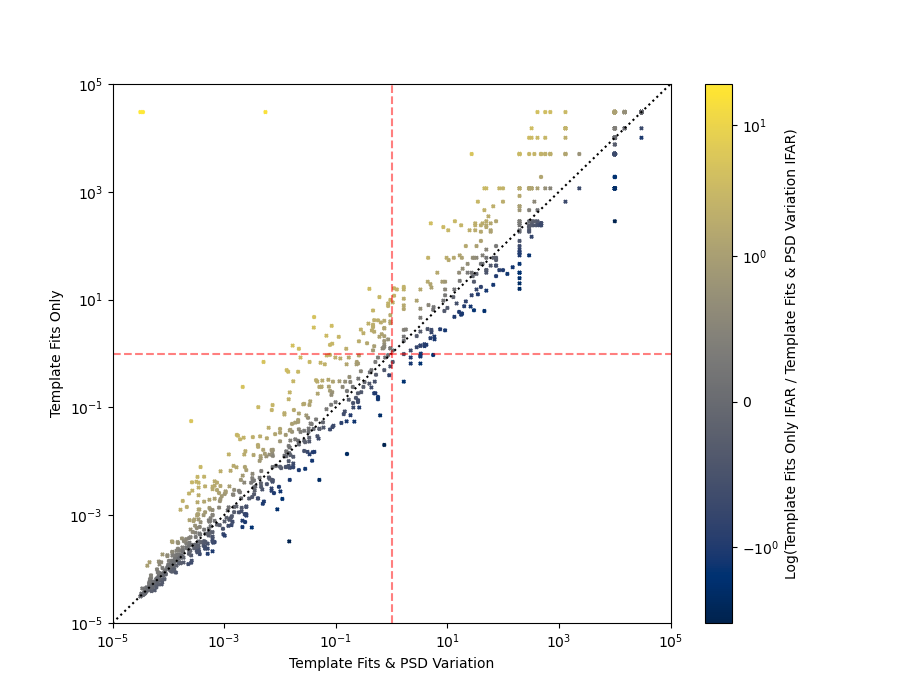
\includegraphics[width=1.2\textwidth]{images/pycbclive/fits_psdvar_comparison_ifar_vs_ifar_diff.png}
    \caption{}
    \label{fig:pycbclive-ifar-ifar-fits-psdvar}
\end{figure}
%
\begin{figure}
  \centering
  \begin{minipage}[t]{0.9\linewidth}
  
    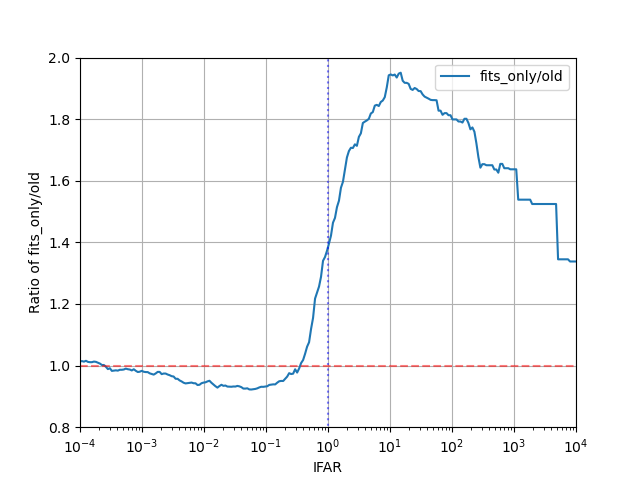
\includegraphics[width=0.9\textwidth]{images/pycbclive/fo_vs_o.png}
    
    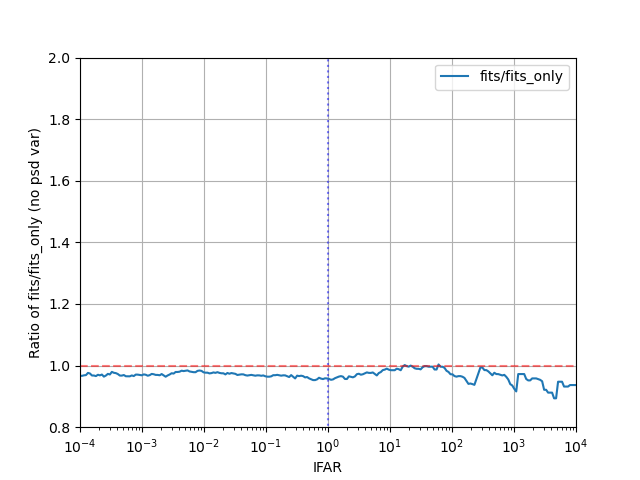
\includegraphics[width=0.9\linewidth]{images/pycbclive/f_vs_fo.png}

  \end{minipage}
  \caption{}
  \label{fig:pycbclive-sensitivity-comparisons}
\end{figure}
%
Figure~\ref{fig:pycbclive-sensitivity-comparisons} (left) shows a marginal increase in sensitivity at the lower IFARs when ignoring PSD variation (compared to figure~\ref{fig:pycbclive-psdvar-4s-sensitivity}) and (right) shows a clear decrease in sensitivity when including the PSD variation in the new statistic search across all IFARs. Therefore we made the choice to not use PSD variation in the PyCBC Live statistic going forward.

\section{\label{pycbclive-investigating-regions}Investigating Downranked Regions}

While we have an overall sensitivity increase (shown by figure~\ref{fig:pycbclive-sensitivity-comparisons}) we have another three regions to investigate after the elimination of the bottom-right blue box, as shown in figure~\ref{fig:pycbclive-ifar-ifar-fits-only-4s}. Once we have investigated these regions and understand the effects of the template fitting on the statistic to cause these downranked events we can be confident in including the template fitting addition in the live ranking statistic.

\subsection{\label{sec:pycbclive-diff-start-times}Different Search Start Times}

While investigating these regions we discovered a very important contribution to the IFAR vs IFAR distribution that we hadn't intended to include in our injection sets. 

To take a step back to explain how this problem was introduced into our data and describe how the initial searches were performed. We have two searches: one with the old statistic, one with the new statistic (including any new components). One of the new components is the template fitting statistic and this required that an additional week of search had to be performed using the old statistic, a week prior to the actual search. Therefore for simplicity we ran the old statistic live search over two weeks with no interruptions and the new statistic live search simply over the second week only, after creating the template fitting files.

The old statistic search began at a GPS time of $1262390400$, with the second week beginning at $1262995020$ so the new statistic search began at this time. The problem is that the difference between the week 1 and week 2 start time ($604,620$) is not divisible by $8$, which is our stride time in live. This means that when the old statistic search is crossing the boundary between week 1 and week 2 it will start week 2 on the stride time $1262995024$ which is four seconds after the offical beginning of week 2.

An easy to see problem is that the old statistic search will have had more initial time to bed in the search, so it had knowledge of the $256$ seconds prior to the start of week 2, we account for this and exclude $256$ seconds of data from the start of both searches. This should prevent the old statistic search from reporting seeing more injections than the new statistic.

A bigger problem is that the live searches are analysing different data as they are searching, there is always going to be a $4$ second difference in the data being analysed at any one time. While both searches will search through the same data (except the old statistic will miss the final $4$ seconds of week 2) the PSD for the $256$ seconds of data being analysed can be different in every stride. All the injections have the potential to be seen with a different SNR due to different noise in the data that is being analysed, therefore while the injections might've been seen with the same template, it was not seen with the same trigger which will change the significance of our injections.

This was discovered when we were seeing different SNR and $\chi^{2}$ values for injections with identical trigger templates and times. Aside from computing issues, our searches should be identical and if they are searching the same data with the same template they should always recover the same values from matched filtering, evidently they weren't due to this mismatch in data.

To solve this problem we re-ran the new statistic search but with the start time being equal to the start time of the old statistic search, $1262995024$. With this re-run search we can re-plot figure~\ref{fig:pycbclive-ifar-ifar-fits-only-4s} now that the same data is being analysed in every stride by both searches, this IFAR vs IFAR plot can be seen in figure~\ref{fig:pycbclive-ifar-ifar-fits-only-0s},
%
\begin{figure}
       \centering
    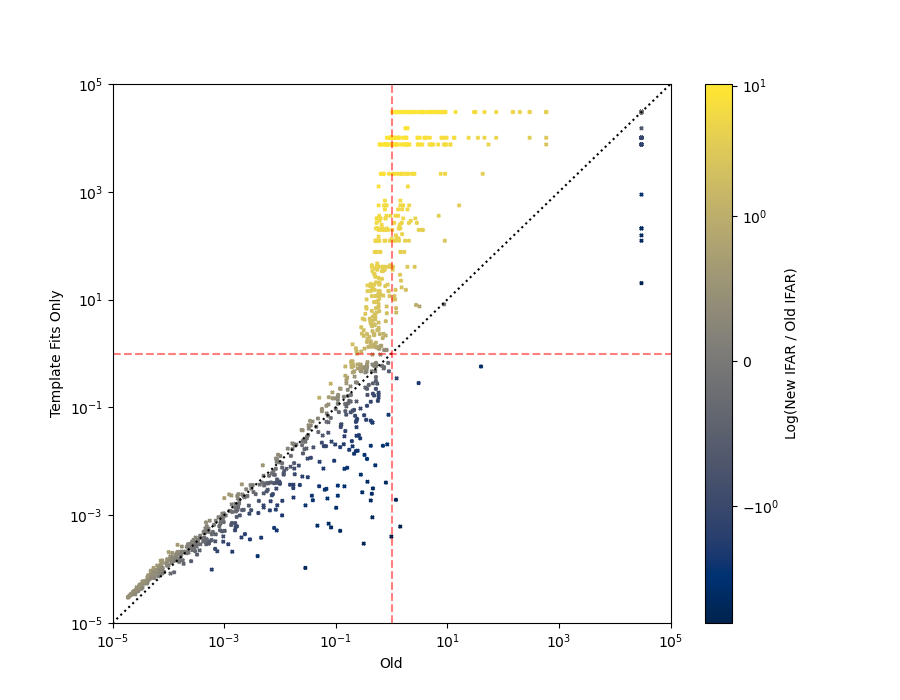
\includegraphics[width=1.2\textwidth]{images/pycbclive/fits_only_0s_ifar_vs_ifar_log_ifar_diff.png}
    \caption{}
    \label{fig:pycbclive-ifar-ifar-fits-only-0s}
\end{figure}
%
and you can see this correction has reduced the spread in the distribution of injections dramatically and is accounting for a lot of the random nature the distribution had in the lower-left quadrant. With this new IFAR vs IFAR plot we are able to re-identify the three regions which will be focus the rest of this section discussing, these regions are highlighted in figure~\ref{fig:pycbclive-ifar-ifar-fits-only-0s}.
%
\begin{figure}
  \centering
  \begin{minipage}[t]{0.9\linewidth}
  
    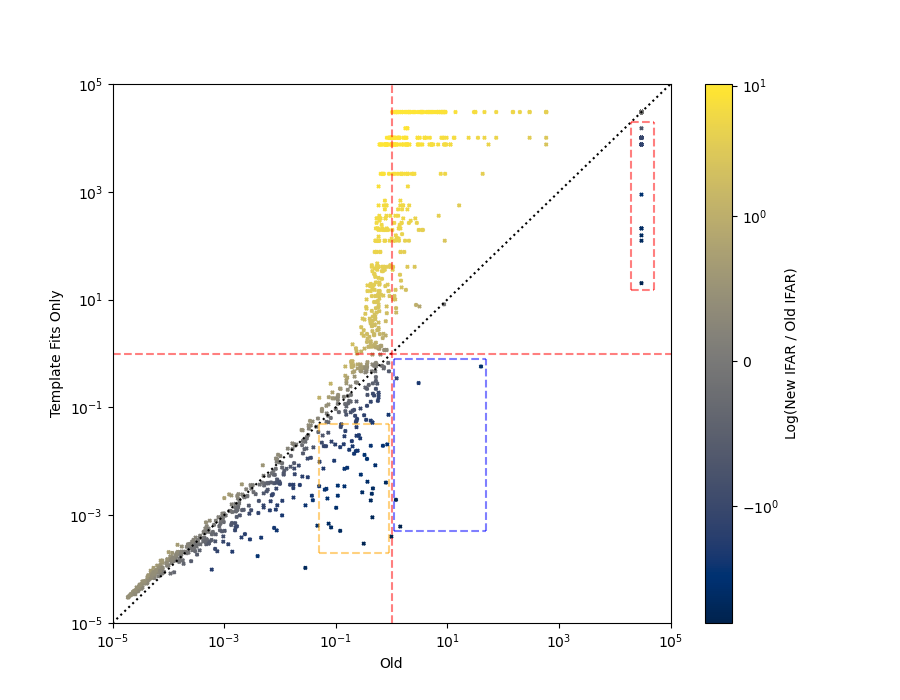
\includegraphics[width=1.2\textwidth]{images/pycbclive/fits_only_0s_ifar_vs_ifar_regions.png}
    \caption{}
    \label{fig:pycbclive-ifar-ifar-fits-only-0s}
    
    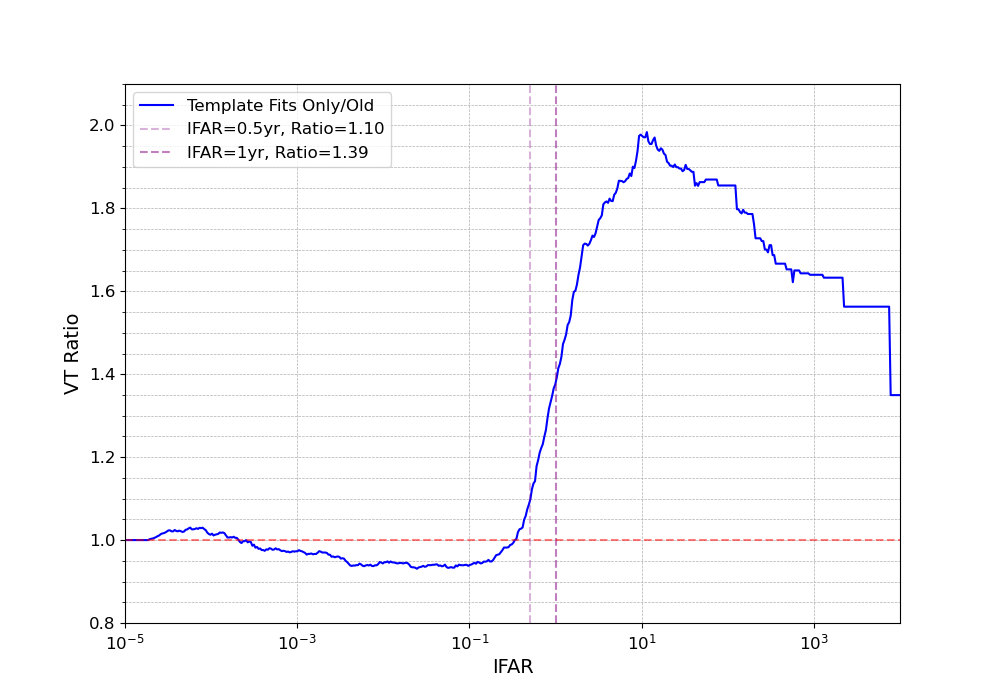
\includegraphics[width=1\textwidth]{images/pycbclive/fits_only_0s_vt_ratio.png}
    \caption{}
    \label{fig:pycbclive-sensitivity-fits-only-0s}

  \end{minipage}
\end{figure}
%
Of the $1275$ jointly observed injections: $704$ are seen with a higher IFAR when including template fits, $309$ with a lower IFAR and, $262$ with the same IFAR. This isn't a complete picture, we don't want to see just an increase in the number of injections with a higher IFAR but higher IFAR values for all out injections. To see this we can look at the VT ratio sensitivity plot, shown in figure~\ref{fig:pycbclive-sensitivity-fits-only-0s}.

%%%%%%%%%%%%%%%%%%%%%%%%%%%%%%%%%%%%%%%%%%%%%%%%%%%%%%%%%%%%
\subsection{\label{sec:pycbclive-poor-temp-fits}Poor Template Fits}

% Log(noise rate) equation
% Combined log(noise rate) equation
% Low Alpha + High Rate == High Combined Log(noise rate)
% Plot Alpha vs Rate, colour Log(noise rate)
% Plot Alpha vs SNR, colour Log(noise rate)

With the inclusion of template fits in the ranking statistic we are now able to model the trigger SNR distributions and abandon the Gaussian noise model previously used. We stop treating all templates equally and can downweight poorly performing templates. In this section we discuss template with poor fits and how we can identify that from the template fit parameters.

All templates in the bank will trigger on noise in our data, from both Gaussian noise and glitches, and after applying all signal consistency tests these triggers might still might have $\rho_{new}$ of over $8$. The template fits are created by collecting all triggers from a template and finding their $\rho_{new}$ distribution--see figure~\ref{fig:pycbclive-template-fits}--and fitting an exponential to this distribution. From this it is possible to qualitatively say that templates which have a large number of high $\rho_{new}$ triggers will have worse fits than those that don't and this is encapsulated in the parameters $\alpha$, the exponential fit factor, and $\mu$, the rate of triggers above some threshold (typically $\rho_{new} = 6.0$ (CHECK)).

These two parameters are then used to re-weight to single detector $\rho_{new}$ and turn it into a noise rate, which we take the natural logarithm of to reduce computational issues surrounding the scale of magnitude difference in these values. The single detector noise rate is given by,
%
\begin{equation}
    r_{d}(\rho_{new}; {\theta}; N) = \mu(\theta) p(\rho | \theta, N) 
\label{eqn:pycbclive-single-noise-rate}
\end{equation}
%
where
%
\begin{equation}
    p(\rho_{new} | \theta, N) = \alpha(\theta) \exp\left(-\alpha(\theta)(\rho_{new} - \rho_{thresh}\right)
\label{eqn:pycbclive-p-definition}
\end{equation}
%
thereby giving the single detector noise rate as,
%
\begin{equation}
    r_{d}(\rho_{new}; {\theta}, N) = \mu(\theta) \alpha(\theta) \exp\left(-\alpha(\theta)(\rho_{new} - \rho_{thresh})\right)
\label{eqn:pycbclive-single-noise-rate-full}
\end{equation}
%
and when the natural logarithm is taken we arrive at the log noise rate equation,
%
\begin{equation}
    ln(r_{d}) = ln(\mu(\theta)) +  ln(\alpha(\theta)) - \alpha(\theta)(\rho_{new} - \rho_{thresh})
\label{eqn:pycbclive-single-log-noise-rate}
\end{equation}
%
for each detector.

Equation~\ref{eqn:pycbclive-single-log-noise-rate} gives us the log noise rate contribution from the single detectors but the combined log noise is what contributes to the ranking statistic (alongside the log signal rate). The combined log noise rate takes into account the noise rates from each detector and also takes into account the `allowed area' for coincidence noise events from two detectors, $A_{N\{12\}} = 2\tau_{12}$, where $\tau_{12}$ is the GW travel time window between detectors 1 \& 2 with a small allowance for timing error (currently $0.002$ seconds). Therefore the entire equation for the combined noise rate is,
%
\begin{equation}
    r_{n} = A_{N} \Pi_{d} r_{d}(\rho_{new})
\label{eqn:pycbclive-comb-noise-rate}
\end{equation}
%
and when the natural logarithm is taken we get the combined log noise rate,
%
\begin{equation}
    ln(r_{n}) = ln(A_{N}) +  \Sigma_{d} ln(r_{d}(\rho_{new}))
\label{eqn:pycbclive-comb-log-noise-rate}
\end{equation}
%
which is used in the ranking statistic calculation. It is therefore plain to see that the $\alpha$ and $\mu$ parameters for each template are directly contributing to the noise rate for an event and equation~\ref{eqn:pycbclive-single-log-noise-rate} shows that low $\alpha$ value and high $\mu$ values are indicative of `poor' fits and cause an elevated noise rate.

This is beneficial when a template frequently triggers on noise and it is downranked in the ranking statistic but it is now possible that real gravitational wave signals belonging to template with poor fits will be downranked if they have lower $\rho_{new}$ values. To help visualise the template fits component contributions in equation~\ref{eqn:pycbclive-single-log-noise-rate} we can plot the single detector log noise rate for a range of $\alpha$ and $\mu$ values, this can be seen in figure~\ref{fig:pycbclive-log-noise-static-snr} where we have used a static $\rho_{new}$ of $10.0$, it can be seen that a higher $\alpha$ value has a great effect on the log noise rate and while $\mu$ has an effect on the log noise rate ($ + \log(\mu)$ in equation~\ref{eqn:pycbclive-single-log-noise-rate}) its contribution is minimal.
%
\begin{figure}
  \centering
  \begin{minipage}[t]{1.0\linewidth}
  
    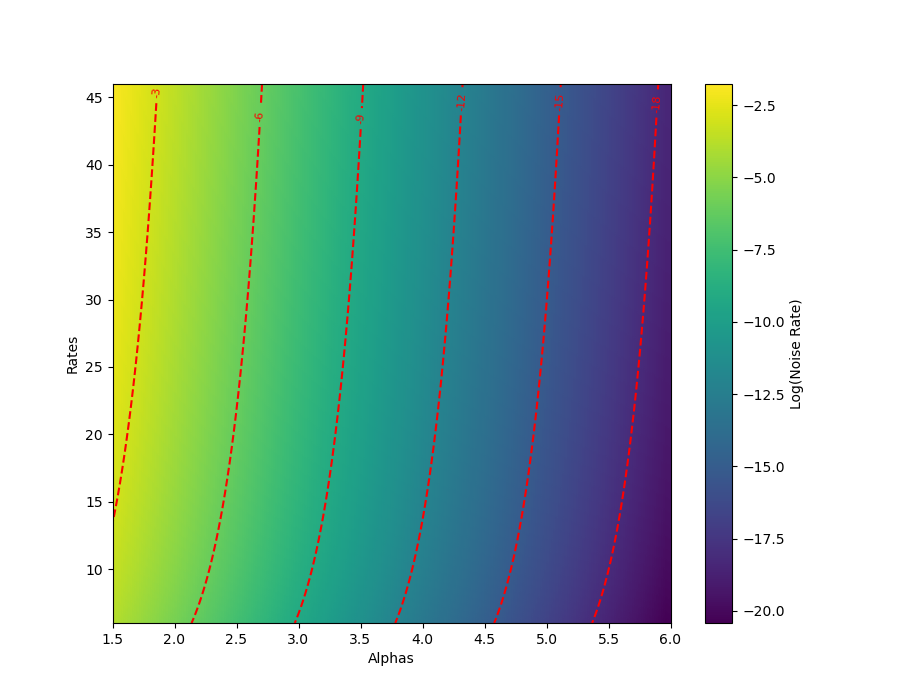
\includegraphics[width=1\textwidth]{images/pycbclive/lognoise_alpha_rate.png}
    \caption{}
    \label{fig:pycbclive-log-noise-static-snr}
  
    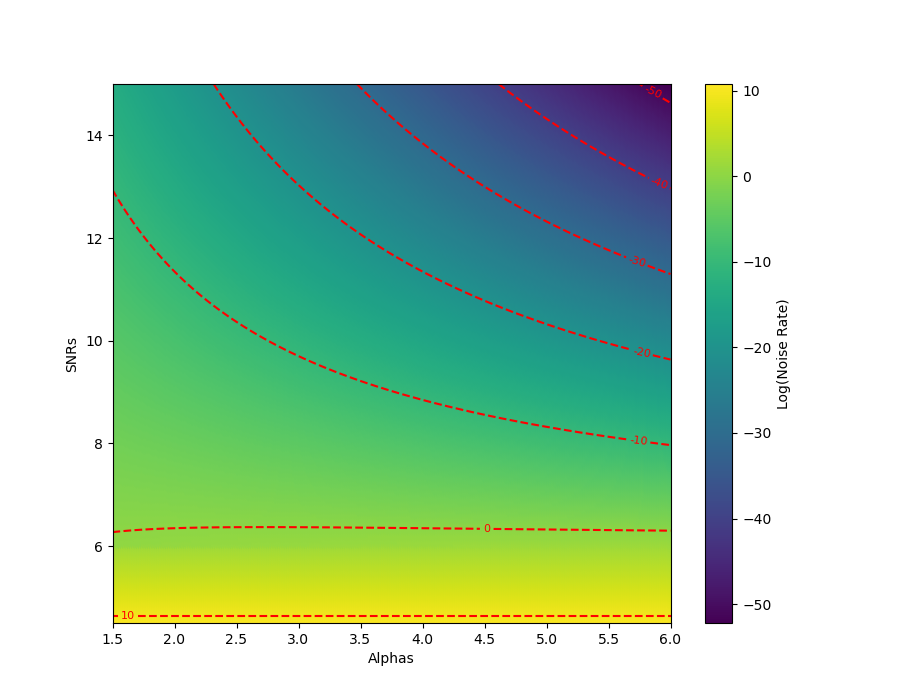
\includegraphics[width=1\textwidth]{images/pycbclive/lognoise_alpha_snr.png}
    \caption{}
    \label{fig:pycbclive-log-noise-static-rate}

  \end{minipage}
\end{figure}
%
We produce the same figure but instead set $\mu$ to the benchmark log noise rate, $-14.6$, which is the log of a representative noise trigger rate and originates from the second observing run, figure~\ref{fig:pycbclive-log-noise-static-rate}. This figure shows us how SNR changes the log noise rate alongisde $\alpha$, a black dashed line has been plotted at $\rho_{new} = 6.0$ due to triggers below this SNR threshold all being assigned $\alpha = 6.0$, therefore the log noise rate values below this threshold are the same for all values on $\alpha$ on our plot. We can clearly see a strong correlation between SNR and log noise rate with a heavy dependency on $\alpha$, to the point where high SNR triggers with `poor' fits (low $\alpha$)--while still significant--are a lot worse than those with `good' fits (high $\alpha$).

From the equation and the plots we can therefore conclude that when comparing the purely $\rho_{new}$ single detector components of the old statistic to the log noise rate including template fits single detector component of the new statistic, there is a very large dependence on template fit parameters in the new statistic. 

% Plot IFAR vs IFAR, colour alpha
% Plot IFAR vs IFAR, colour rate
% Plot IFAR vs IFAR, colour H1 log(noise rate)
% Plot IFAR vs IFAR, colour L1 log(noise rate)
% Plot IFAR vs IFAR, colour Combined log(noise rate)

We can plot the IFAR vs IFAR distribution for the injection set for a single detector's $\alpha$, $\mu$ and log noise rate to see if there is any clear dependence on the template fit parameters, seen in figures~\ref{fig:pycbclive-ifar-ifar-h1-alpha},~\ref{fig:pycbclive-ifar-ifar-h1-rate}, and~\ref{fig:pycbclive-ifar-ifar-h1-log-noise-rate}.
%
\begin{figure}
    \centering
    \begin{minipage}[t]{0.8\textwidth}
        \centering
        \vspace{-0.75cm}
        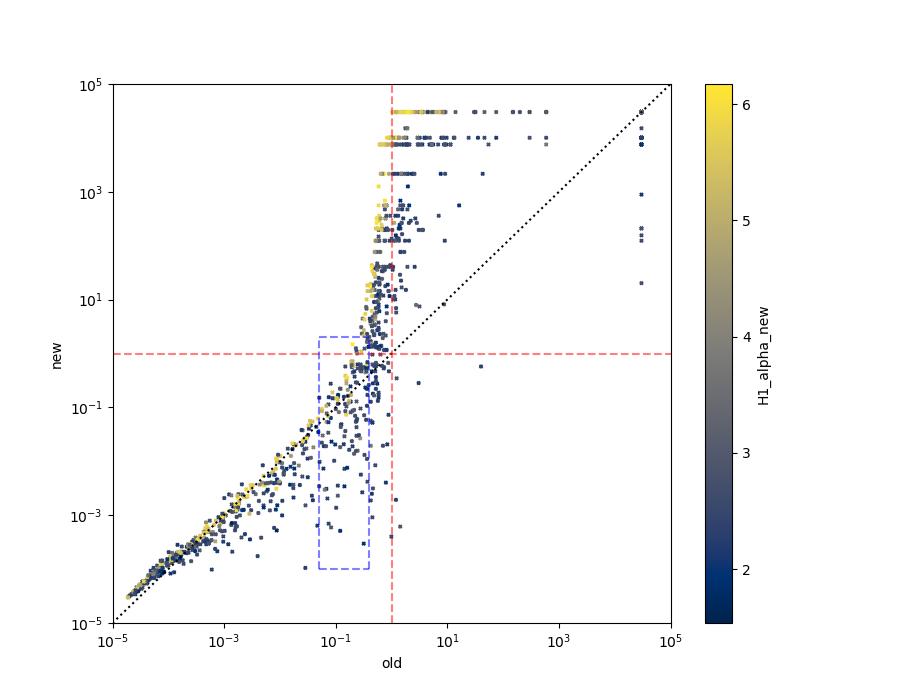
\includegraphics[width=\textwidth]{images/pycbclive/all_full_h1_alpha.png}
        \caption{}
        \label{fig:pycbclive-ifar-ifar-h1-alpha}
        \vspace{-0.95cm}
        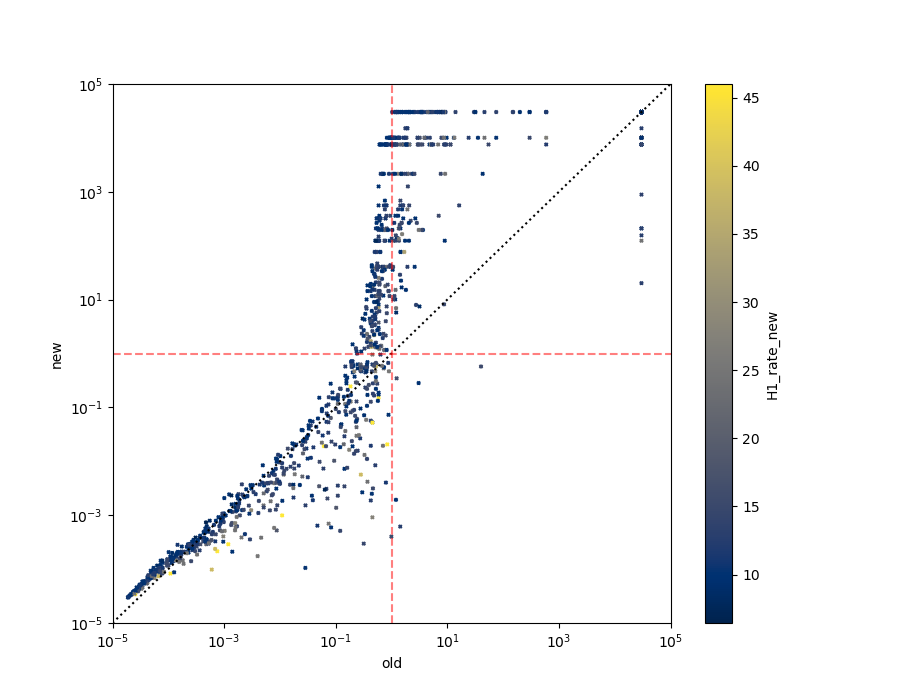
\includegraphics[width=\textwidth]{images/pycbclive/all_full_h1_rate.png}
        \caption{}
        \label{fig:pycbclive-ifar-ifar-h1-rate}
        \vspace{-0.95cm}
        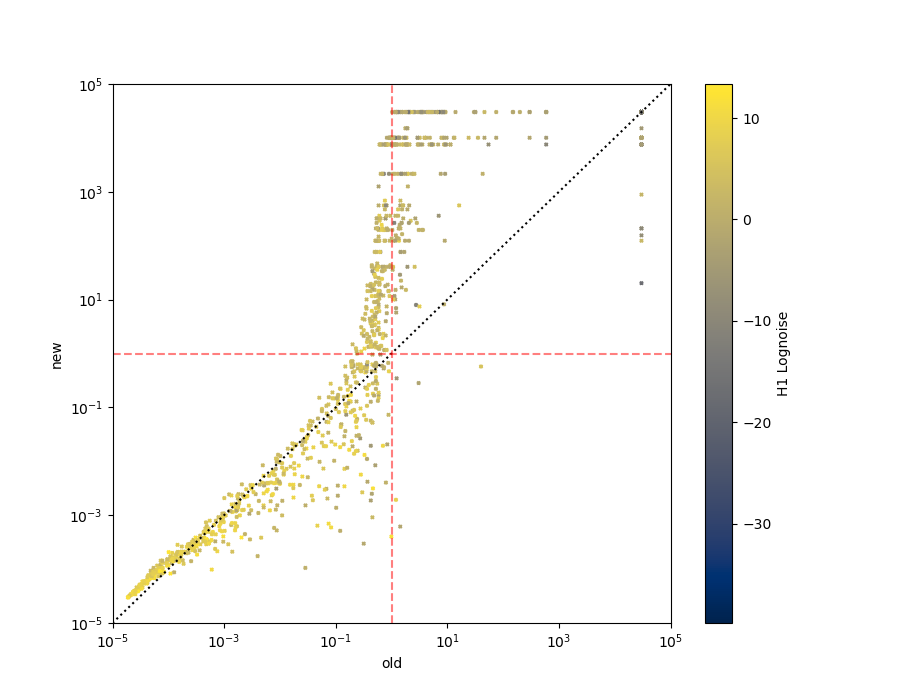
\includegraphics[width=\textwidth]{images/pycbclive/all_full_h1_lognoise.png}
        \caption{}
        \label{fig:pycbclive-ifar-ifar-h1-log-noise-rate}
    \end{minipage}
\end{figure}
%
It is not clear from these figures that $\alpha$ and $\mu$ are having a large effect on the log noise shown in the bottom figure. There is a curve of high $\alpha$ points above the $y=x$ line in the top figure but we would hope to see a better distinction between higher and lower $\alpha$ values corresponding to improved and worsened IFAR values. As mentioned before and reinforced by the middle plot, the rate has a small effect on the log noise rate and low rate values are far more common than high ones, the high ones are located in the bottom left quadrant below the $y=x$ line.

To investigate this further we can look at the distribution of combined log noise rates, shown in figure~\ref{fig:pycbclive-ifar-ifar-comb-log-noise-rate}.
%
\begin{figure}
  \centering
  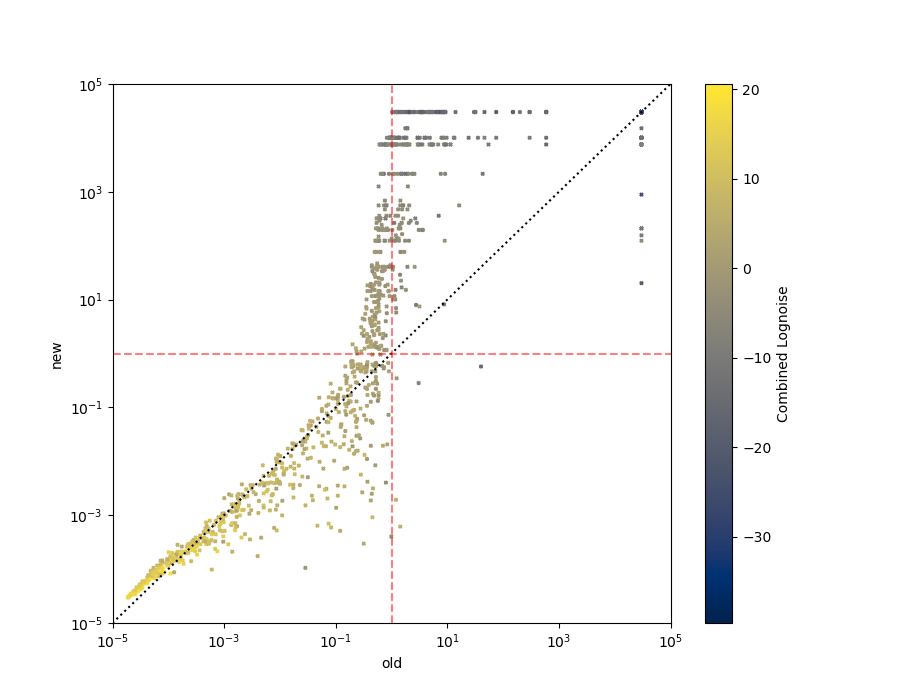
\includegraphics[width=1\textwidth]{images/pycbclive/all_full_comb_lognoise.png}
  \caption{}
  \label{fig:pycbclive-ifar-ifar-comb-log-noise-rate}
\end{figure}
%
From this figure we can see a much clearer distinction between higher and lower noise rates and how this is affecting the ranking statistic, where we expect a lower noise rate to improve the ranking statistic. However, looking at this plot we can see that combined log noise rate isn't the entire explanation for improved significance, we can see clearly there are some low noise rate injections below the $y=x$ line which should have caused an increase in the significance but we have seen a drop. Therefore we must investigate other components of the ranking statistic and how these build up our ranking statistic model.

\subsection{\label{sec:pycbclive-diff-triggers}Different Triggers Selected by Each Search}

% Different triggers == different templates
% Different templates == different signal rate
% Plots of same trigger
% Plots of different trigger
% Plots of Total Ranking Statistic distribution

The inclusion of the template fits will quantitatively change how the combined noise rate contributes to the ranking statistic but, there is another component to the ranking statistic that can change. Our ranking statistic is a simple sum of four separate components, the two that can change are the combined log noise rate and the log signal rate, therefore we can reduce the new statistic ranking statistic equation simply to $R = log(r_s) - log(r_n)$.

Therefore we can look at the scenario where the log signal rate has also changed between searches. The log signal rate is dependent on four parameters of a trigger: $\rho$ (note, not $\rho_{new}$), $\phi$, $t_{c}$ and, $\verb|sigmasq|$. We expect the phase, $\phi$, and time, $t_{c}$, differences between detectors to be determined by the detector's location and the source's sky location and orientation. Therefore, for a particular trigger we expect this to be the same in both searches and the log signal rate would be the same for the same trigger.

If we see a different trigger between searches this opens up potential for a difference in the log signal rate to effect the ranking statistic. However, this also poses the question of why the search has chosen a different trigger between searches? The event with the highest ranking statistic is chosen as the best event for a particular injection and therefore we come back to the specific components of the ranking statistic changing between searches but also the formulation of the ranking statistic itself. 

% Changes in ranking statistic, balance between logr_s and logr_n
% Plot signal rate for same trigger, IFAR vs IFAR
% Plot signal rate for different trigger, IFAR vs IFAR
% Plot new ranking statistic total, IFAR vs IFAR
% Plot old ranking statistic total, IFAR vs IFAR

We can directly compare the equation for the old ranking statistic,
%
\begin{equation}
    R_{old} = \sqrt{2(ln(r_n) + ln(r_s))}
\label{eqn:pycbclive-old-ranking-statistic}
\end{equation}
%
to that of the new ranking statistic,
%
\begin{equation}
    R_{new} =  ln(r_s) - ln(r_n)
\label{eqn:pycbclive-new-ranking-statistic-simple}
\end{equation}
%
and we can immediately see a clear difference in how both the noise rates and signal rates contribute to the ranking statistic value. It is due to these formulations that we cannot directly compare ranking statistic values between searches to identify why the significance of injections has changed.

Different triggers in the new statistic search have therefore been found with a higher ranking statistic when compared to the trigger found by the original search, an example of one of these is seen in table~\ref{tab:pycbclive-200-new-stat},
%TABLE
%
\begin{table}[ht]
    \centering
    \setlength{\tabcolsep}{3pt}
    \begin{minipage}{0.48\textwidth}
        \centering
        \rowcolors{2}{white}{lightgray}
        \begin{adjustbox}{minipage=\linewidth-0cm, margin=-5.5cm 0pt 0pt 0cm}
        \begin{tabular}{lcc}
            \toprule
            \textbf{Inj Idx = 200} & \textbf{Old Trigger} & \textbf{New Trigger} \\
            \midrule
            Comb Log(Noise Rate)  & -15.53 & -18.79 \\
            Log(Signal Rate) & -15.77 & -15.67 \\
            $R_{new}$ & -0.24 & 3.12 \\
            \bottomrule
        \end{tabular}
        \end{adjustbox}
        \caption{}
        \label{tab:pycbclive-200-new-stat}
    \end{minipage}
    \hfill
    \begin{minipage}{0.48\textwidth}
        \centering
        \rowcolors{2}{white}{lightgray}
        \begin{tabular}{lcc}
            \toprule
            \textbf{Inj Idx = 445} & \textbf{Old Trigger} & \textbf{New Trigger} \\
            \midrule
            Comb Log(Noise Rate)  & -12.96 & -12.69 \\
            Log(Signal Rate) & -4.40 & -2.74 \\
            $R_{new}$ & 8.56 & 9.95 \\
            \bottomrule
        \end{tabular}
        \caption{}
        \label{tab:pycbclive-445-new-stat}
    \end{minipage}
\end{table}
%
It can be seen that the signal rate contribution is marginally improved in the new trigger but the noise rate contribution is the majority of the increase in the ranking statistic. Table~\ref{tab:pycbclive-445-new-stat} shows a different case where the noise rates of the old and new trigger are similar but by selecting a different template we have found an improved signal rate causing the increase in the ranking statistic. We can also show the ranking statistic values found by the old statistic to see why these triggers are different, tables~\ref{tab:pycbclive-200-old-stat} and~\ref{tab:pycbclive-445-old-stat} show these.
%TABLE
%
\begin{table}[ht]
    \centering
    \setlength{\tabcolsep}{5pt}
    \begin{minipage}{0.48\textwidth}
        \centering
        \rowcolors{2}{white}{lightgray}
        \begin{adjustbox}{minipage=\linewidth-0cm, margin=-5cm 0pt 0pt 0cm}
        \begin{tabular}{lcc}
            \toprule
            \textbf{Inj Idx = 200} & \textbf{Old Trigger} & \textbf{New Trigger} \\
            \midrule
            $\rho_{new, H1}$  & 15.06 & 13.50 \\
            $\rho_{new, L1}$   & 6.67 & 6.58 \\
            $\rho_{new, H1}^2 + \rho_{new, L1}^2$   & 271.29 & 225.25 \\
            Log(Signal Rate) & -15.77 & -15.67 \\
            $R_{new}$ & 15.48 & 13.93 \\
            \bottomrule
        \end{tabular}
        \end{adjustbox}
        \caption{}
        \label{tab:pycbclive-200-old-stat}
    \end{minipage}%
    \hfill
    \begin{minipage}{0.48\textwidth}
        \centering
        \rowcolors{2}{white}{lightgray}
        \begin{tabular}{lcc}
            \toprule
            \textbf{Inj Idx = 445} & \textbf{Old Trigger} & \textbf{New Trigger} \\
            \midrule
            $\rho_{H1,new}$  & 10.44 & 10.78 \\
            $\rho_{L1,new}$   & 8.14 & 7.16 \\
            $\rho_{H1,new}^2 + \rho_{L1,new}^2$   & 175.25 & 167.47 \\
            Log(Signal Rate) & -4.40 & -2.74 \\
            $R_{new}$ & 12.90 & 12.73 \\
            \bottomrule
        \end{tabular}
        \caption{}
        \label{tab:pycbclive-445-old-stat}
    \end{minipage}
\end{table}
%
We can plot the IFAR vs IFAR distribution with the combined log signal rate as the colour of each injection but we can further split this into two groups, those found with the same trigger in both searches (figure~\ref{fig:pycbclive-ifar-ifar-same-trigs-comb-log-noise-rate}) and those found with different triggers figure~\ref{fig:pycbclive-ifar-ifar-diff-trigs-comb-log-noise-rate}. These plots show there is no clear difference in the combined log noise values associated with injections found with the same or different triggers between searches.
% PLOT
% SAME TRIGGER, LOG SIG RATE
% DIFF TRIGGER, LOG SIG RATE
%
\begin{figure}
  \centering
  \begin{minipage}[t]{1.0\linewidth}
  
    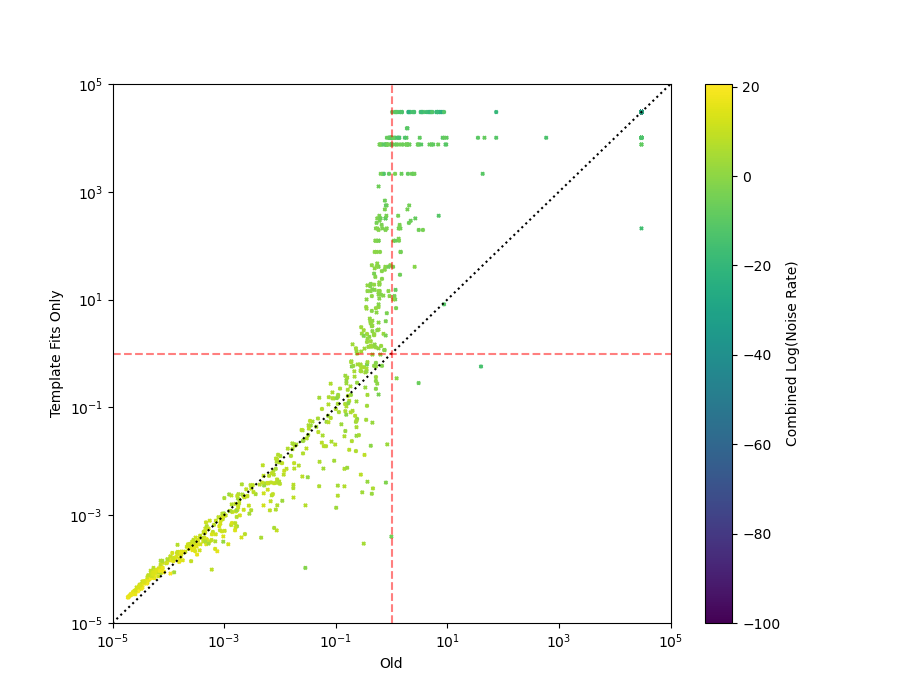
\includegraphics[width=1\textwidth]{images/pycbclive/ifar_vs_ifar_same_template_ids_comb_log_noise.png}
    \caption{}
    \label{fig:pycbclive-ifar-ifar-same-trigs-comb-log-noise-rate}
  
  % \hspace{0.01\linewidth}
  
    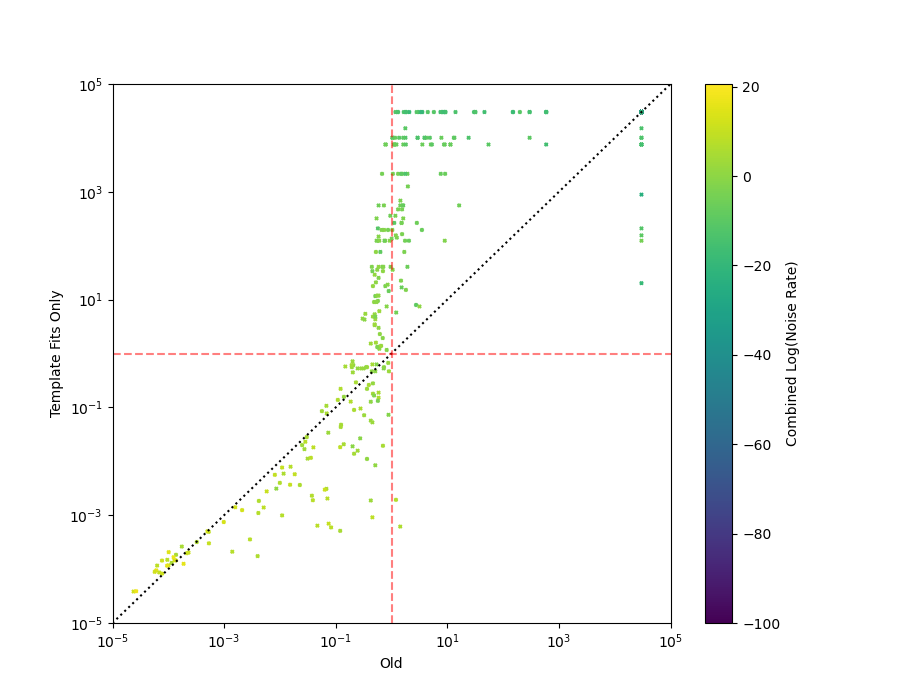
\includegraphics[width=1\textwidth]{images/pycbclive/ifar_vs_ifar_diff_template_ids_comb_log_noise.png}
    \caption{}
    \label{fig:pycbclive-ifar-ifar-diff-trigs-comb-log-noise-rate}
  
  \end{minipage}
\end{figure}
%
Another plot we can look into is how these injections are distributed in both the old and new ranking statistic values. Figures~\ref{fig:pycbclive-ifar-ifar-old-stat} and~\ref{fig:pycbclive-ifar-ifar-new-stat} show the IFAR vs IFAR plot with the top plot showing the injections coloured with their old statistic value and the bottom plot showing them coloured with their new statistic value. The progression of the colours can be seen as corresponding to the $x$ and $y$ directions as plotted, this is because there is a direct mapping between ranking statistic and IFAR for each search. In both figures, ranking statistic values above the colourbar max were set equal to the max to prevent large ranges of statistic values drowning out the smaller differences.
% PLOT
% OLD STAT
% NEW STAT
%
\begin{figure}
  \centering
  \begin{minipage}[t]{1.0\linewidth}
  
    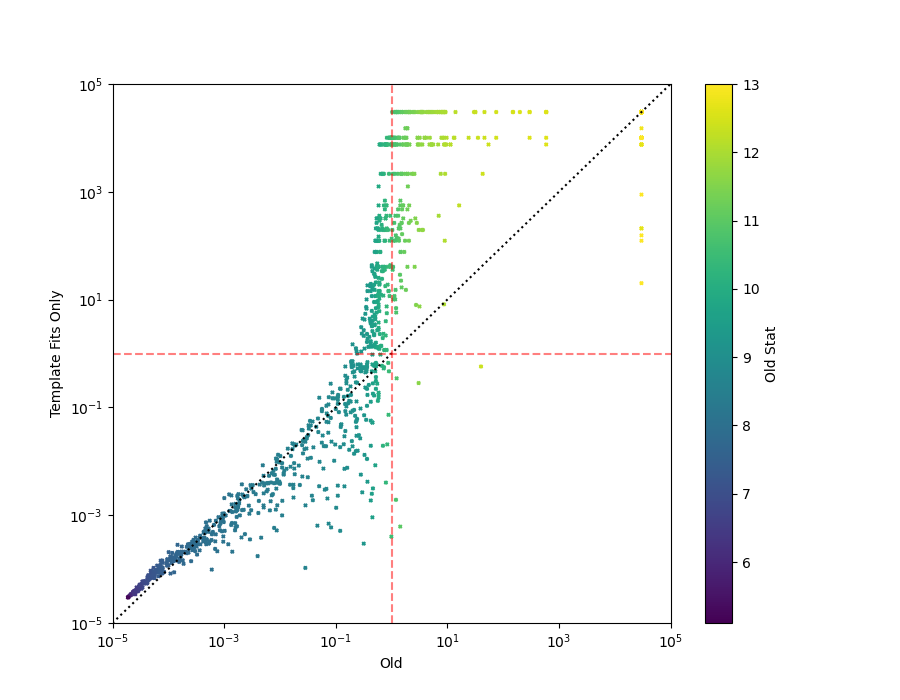
\includegraphics[width=1\textwidth]{images/pycbclive/ifar_vs_ifar_old_stat.png}
    \caption{}
    \label{fig:pycbclive-ifar-ifar-old-stat}
  
  % \hspace{0.01\linewidth}
  
    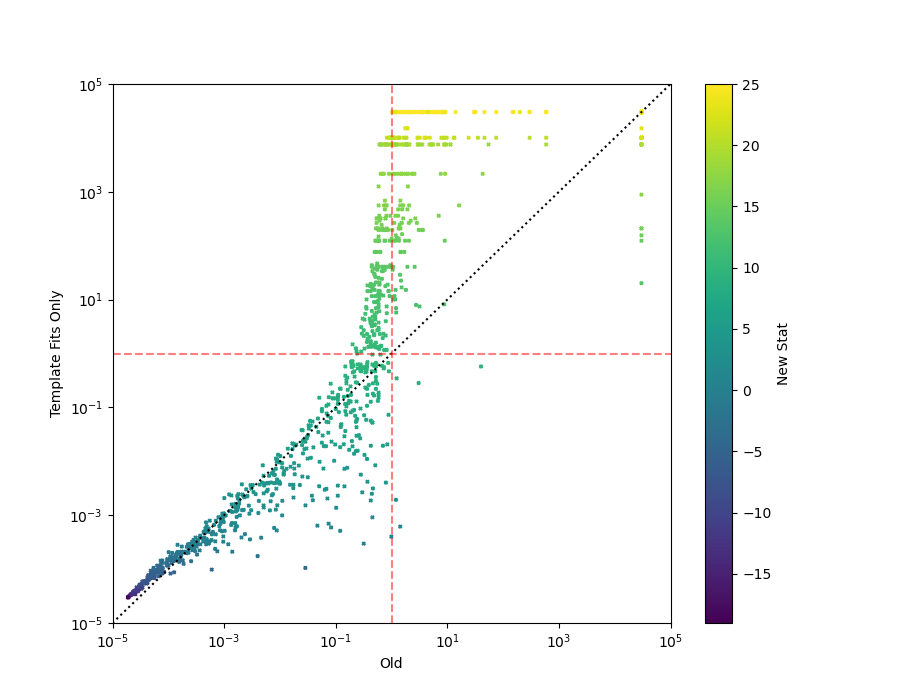
\includegraphics[width=1\textwidth]{images/pycbclive/ifar_vs_ifar_new_stat.png}
    \caption{}
    \label{fig:pycbclive-ifar-ifar-new-stat}
  
  \end{minipage}
\end{figure}
%



\subsection{\label{sec:pycbclive-noise-contrib}Differences in the Noise Rate Contribution}

% Old Statistic Noise Rate

The old statistic assumes Gaussian, stationary noise for the noise rate. Therefore, we can model the noise rate for each detector as a Gaussian distribution,
%
\begin{equation}
    r_{n,det} \propto \exp \left( -\frac{(\rho_d - \mu)^2}{2 \sigma^2} \right)
    \label{eqn:pycbclive-old-noise-rate}
\end{equation}
%
and the combined noise rate is the product of both detector noise rates,
%
\begin{equation}
    r_{n,comb} \propto \exp \left( -\frac{(\rho_{H}^{2} + \rho_{L}^{2})}{2} \right) ,
    \label{eqn:pycbclive-old-comb-noise-rate}
\end{equation}
%
when the mean is equal to 0 and the variance 1. It can be seen from equation~\ref{eqn:pycbclive-old-comb-noise-rate} that the the rate of noise events decreases exponentially with the sum of the SNR$^{2}$s of the triggers.

% New Statistic Noise Rate
The new statistic attempts to model the distribution of the noise events using template fits and therefore the noise is not assumed to be Gaussian or stationary. We can plot the combined log noise rate (equation~\ref{eqn:pycbclive-comb-log-noise-rate}) as a function of detector SNR with the old statistic combined log noise rate shown in figure~\ref{fig:pycbclive-comb-lognoise-old} and the new statistic in figure~\ref{fig:pycbclive-comb-lognoise-new}.
%
\begin{figure}
  \centering
  \begin{minipage}[t]{1.0\linewidth}
  
    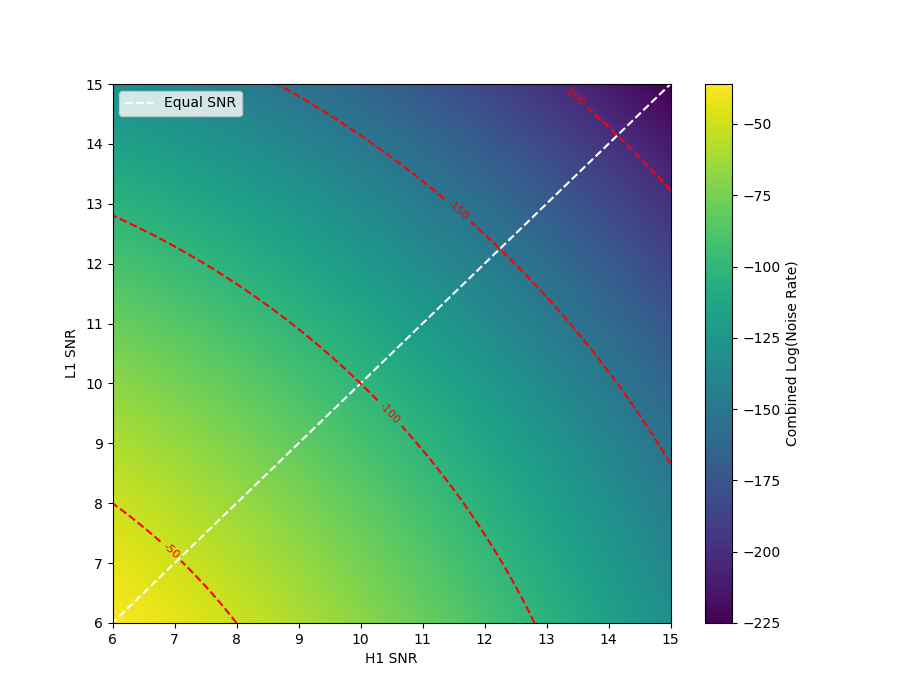
\includegraphics[width=1\textwidth]{images/pycbclive/comb_lognoise_old_stat.png}
    \caption{}
    \label{fig:pycbclive-comb-lognoise-old}
  
  % \hspace{0.01\linewidth}
  
    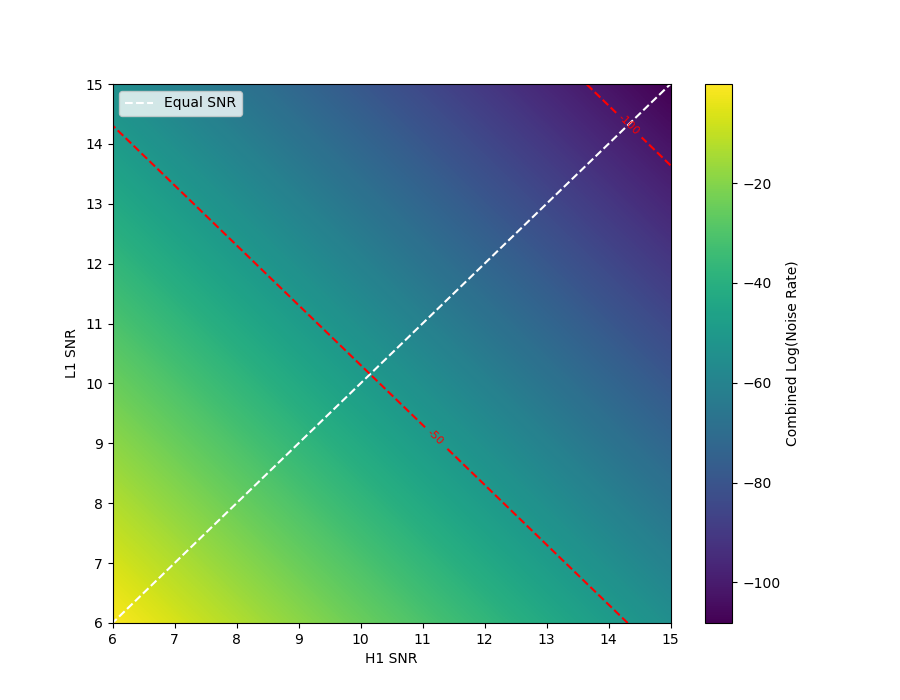
\includegraphics[width=1\textwidth]{images/pycbclive/comb_lognoise_new_stat.png}
    \caption{}
    \label{fig:pycbclive-comb-lognoise-new}
  
  \end{minipage}
\end{figure}
%
The old statistic has a distinct curvature in the combined log noise rate contours which is a result of the Gaussian noise model we are using. The new statistic doesn't have this curvature. Note, the combined log noise rate values cannot be directly compared between statistics.

One particular way this noise rate model difference manifests is in the ratio of the two detector $\rho_{new}$ values. The Gaussian model attempts to maximise the squared sum of the SNR values from each detector with only the signal-consistency tests to weight the new SNR. Our new model adds additional weights in the form of the template fits so that if a different trigger is seen with slightly less SNR in both detectors but the template has much better fits, then it will be preferred by the log noise rate model. Figure~\ref{fig:pycbclive-ifar-ifar-snr-ratio} shows the injections coloured by the SNR ratio in the new statistic search.
%
\begin{figure}
  \centering
  \begin{minipage}[t]{1.0\linewidth}
    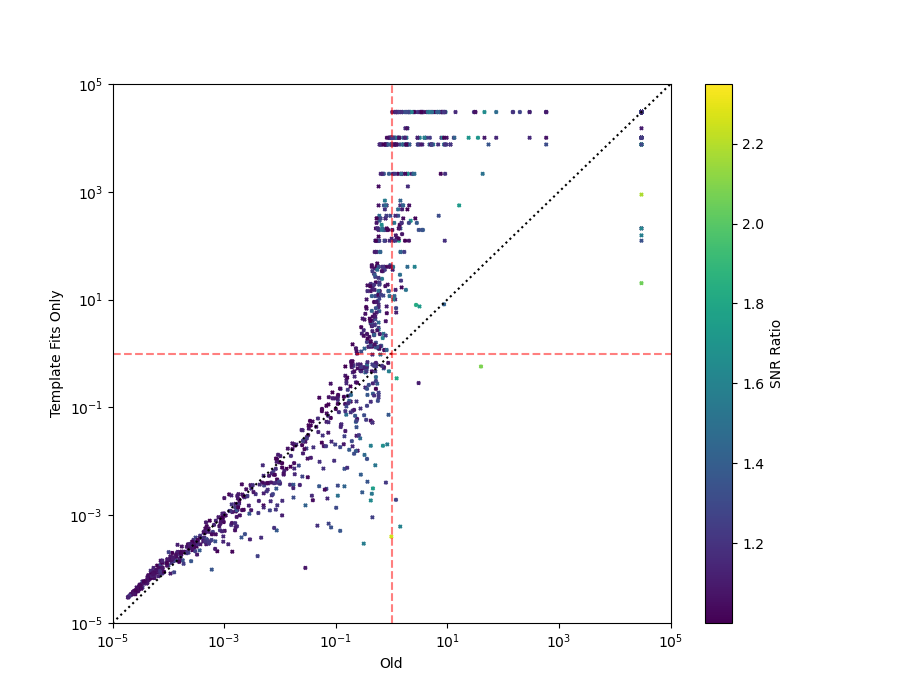
\includegraphics[width=1\textwidth]{images/pycbclive/ifar_vs_ifar_snr_ratio_new.png}
  \end{minipage}
  \caption{}
  \label{fig:pycbclive-ifar-ifar-snr-ratio}
\end{figure}
%
It can be seen that there are a number of points in regions of interest (figure~\ref{fig:pycbclive-ifar-ifar-fits-only-0s}) that have been downranked by the new search specifically because they have a high SNR ratio in the old statistic.

\subsection{\label{sec:pycbclive-top-right}Reduced Significance of Previously Highly Significant Injections}

The first region to investigate is the red box in the top-right corner of figure~\ref{fig:pycbclive-ifar-ifar-fits-only-0s}. These are injections that were found with the maximum significance by the old statistic but they have been downranked by the inclusion of template fitting in the ranking statistic. While they have been downranked, they are still all found with a high significance above threshold. 

This region contains $24$ injections, which we can split into two groups for investigation: $12$ injections found with the same trigger in both searches and $12$ injections found with different triggers in both searches. Figure~\ref{fig:pycbclive-top-right-region} shows the distribution of same and different trigger injections in the region, it can be seen that both groups overlap and there isn't a distinct population difference.
%
\begin{figure}
       \centering
    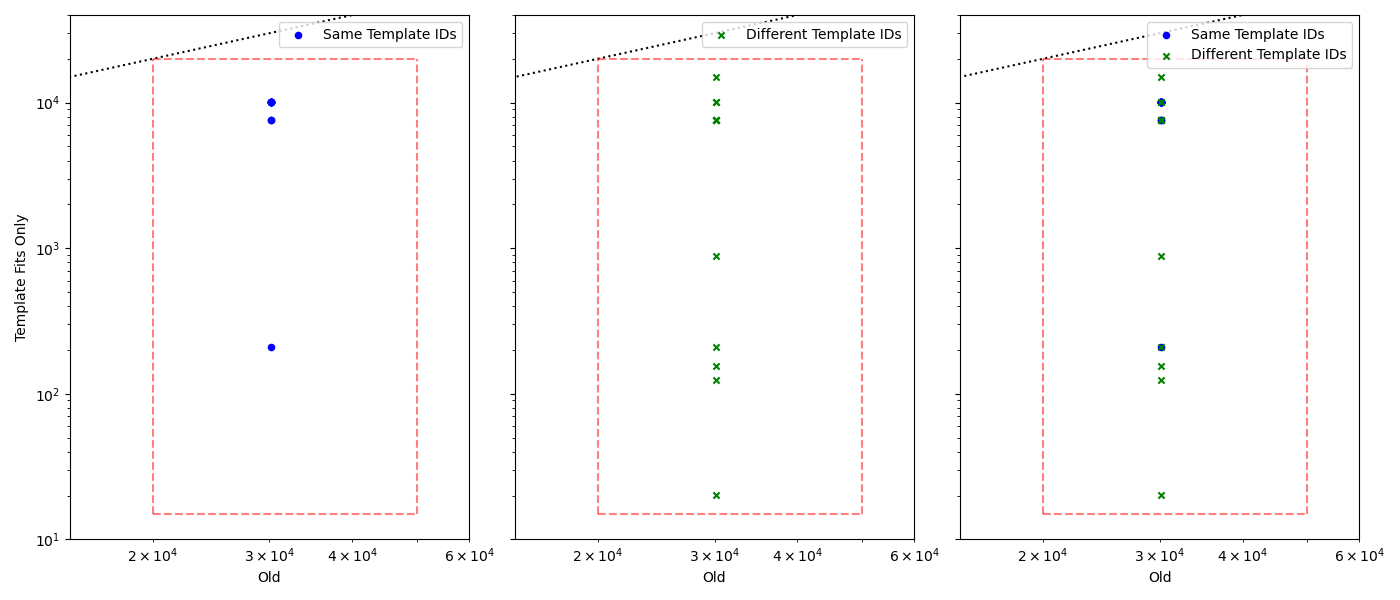
\includegraphics[width=1\textwidth]{images/pycbclive/ifar_vs_ifar_subplots.png}
    \caption{}
    \label{fig:pycbclive-top-right-region}
\end{figure}
%
% Same Triggers
When an injection is found with the same trigger across both searches we can dismiss any changes in $\rho_{new}$ being the cause for an IFAR drop and focus solely on the previously discussed changes like poor template fits and noise rate contribution changes.

First we must double check these were found with identical SNR and $\chi^{2}$ values, this was how we discovered the time discrepancy described in section~\ref{sec:pycbclive-diff-start-times}. Table~\ref{tab:pycbclive-same-trigs-snr-chi} shows $5$ of the $12$ injections and their single detector parameters where it can be plainly seen that these are consistent between searches. This is true for the other $7$ injections also.
%
\begin{table}[ht]
    \centering
    % \small
    \setlength{\tabcolsep}{5pt}
    \begin{tabular}{|l|c|c|c|c|c|c|c|c|c|c|c|c|}
        \toprule
        & \multicolumn{6}{c|}{New} & \multicolumn{6}{c|}{Old} \\
        \hline
        & \multicolumn{3}{c|}{H1} & \multicolumn{3}{c|}{L1} & \multicolumn{3}{c|}{H1} & \multicolumn{3}{c|}{L1} \\
        \hline
        \textbf{Inj Idx} & \textbf{SNR} & \textbf{$\chi^{2}$} & \textbf{SG} & \textbf{SNR} & \textbf{$\chi^{2}$} & \textbf{SG} & \textbf{SNR} & \textbf{$\chi^{2}$} & \textbf{SG} & \textbf{SNR} & \textbf{$\chi^{2}$} & \textbf{SG} \\
        \hline
        1 & 1.1 & 2.2 & 3.3 & 4.4 & 5.5 & 6.6 & 1.1 & 2.2 & 3.3 & 4.4 & 5.5 & 6.6 \\
        2 & 1.1 & 2.2 & 3.3 & 4.4 & 5.5 & 6.6 & 1.1 & 2.2 & 3.3 & 4.4 & 5.5 & 6.6 \\
        3 & 1.1 & 2.2 & 3.3 & 4.4 & 5.5 & 6.6 & 1.1 & 2.2 & 3.3 & 4.4 & 5.5 & 6.6 \\
        4 & 1.1 & 2.2 & 3.3 & 4.4 & 5.5 & 6.6 & 1.1 & 2.2 & 3.3 & 4.4 & 5.5 & 6.6 \\
        5 & 1.1 & 2.2 & 3.3 & 4.4 & 5.5 & 6.6 & 1.1 & 2.2 & 3.3 & 4.4 & 5.5 & 6.6 \\
        \bottomrule
    \end{tabular}
    \caption{Sample data with new and old metrics}
    \label{tab:pycbclive-same-trigs-snr-chi}
\end{table}
%
Looking at the template fit parameter values for the triggers themselves is the first step in identifying any `poor' fits. We can look at the $\rho_{new}$, $\alpha$ and $\mu$ values of each of the $12$ same trigger injections and calculate the single detector log noise rate, these values can be seen in table~\ref{tab:pycbclive-top-right-same-trigs-fits}, alongside the combined log noise rate, log signal rate (which is equal in both searches for the same trigger injections) and the ranking statistic value (calculated simply using $R = ln(r_s) - Comb. ln(r_n)$).
%
\begin{table}[ht]
    \centering
    \small
    \setlength{\tabcolsep}{5pt}
    \rowcolors{2}{white}{lightgray}
    \begin{adjustbox}{minipage=\linewidth-0cm, margin=-4cm 0pt 0pt 0cm}
    \begin{tabular}{lccccccccccc}
        \toprule
        & \multicolumn{4}{c}{\textbf{H1}} & \multicolumn{4}{c}{\textbf{L1}} \\
        \cmidrule(lr){2-5} \cmidrule(lr){6-9}
        \textbf{Inj Idx} & \textbf{$\rho_{new}$} & \textbf{$\alpha$} & \textbf{$\mu$} & \textbf{ln(r$_n$)} & \textbf{$\rho_{new}$} & \textbf{$\alpha$} & \textbf{$\mu$} & \textbf{ln(r$_n$)} & \textbf{Comb. ln(r$_n$)} & \textbf{ln(r$_s$)} & \textbf{Rank. Stat.} \\
        \midrule
        8015 & 8.53 & 2.60 & 24.5 & -2.42 & 9.35 & 2.75 & 22.5 & -5.07 & -11.22 & 0.55 & 11.77 \\
        8026 & 9.31 & 2.37 & 9.4 & -4.74 & 8.88 & 2.52 & 14.4 & -3.67 & -12.14 & -0.91 & 11.23 \\
        8110 & 8.99 & 2.37 & 9.4 & -3.97 & 10.30 & 2.52 & 14.4 & -7.26 & -14.96 & -4.78 & 10.18 \\
        9222 & 10.09 & 2.78 & 15.0 & -7.63 & 9.11 & 2.63 & 23.0 & -4.07 & -15.44 & -3.04 & 12.40 \\
        9365 & 7.34 & 2.57 & 24.0 & 0.68 & 10.88 & 2.28 & 29.0 & -6.94 & -9.99 & 0.14 & 10.13 \\
        9777 & 8.33 & 2.57 & 33.75 & -1.51 & 9.30 & 2.78 & 34.25 & -4.63 & -9.86 & 1.91 & 11.77 \\
        10105 & 9.23 & 2.01 & 13.67 & -3.18 & 8.89 & 2.95 & 20.0 & -4.46 & -11.37 & -0.31 & 11.06 \\
        10251 & 9.52 & 2.37 & 9.4 & -5.23 & 10.26 & 2.52 & 14.4 & -7.17 & -16.14 & -10.22 & 5.92 \\
        10979 & 8.31 & 2.01 & 13.67 & -1.33 & 10.23 & 2.95 & 20.0 & -8.41 & -13.47 & -2.02 & 11.45 \\
        11386 & 12.34 & 2.37 & 9.4 & -11.91 & 6.47 & 2.52 & 14.4 & 2.41 & -13.22 & -5.02 & 8.20 \\
        11608 & 9.93 & 1.93 & 14.5 & -4.24 & 7.68 & 2.83 & 23.75 & -0.56 & -8.52 & 1.07 & 9.59 \\
        13845 & 8.40 & 2.37 & 9.4 & -2.57 & 10.37 & 2.52 & 14.4 & -7.44 & -13.74 & -1.53 & 12.21 \\
        \bottomrule
    \end{tabular}
    \end{adjustbox}
    \caption{}
    \label{tab:pycbclive-top-right-same-trigs-fits}
\end{table}
%
To demonstrate how the addition of template fits can cause the downranking of an injections we pick injection $10251$ which had the most significant drop, from maximum IFAR in the old statistic to an IFAR of $209.55$ years when found with the new statistic. We display the ranking statistic components for both searches in tables~\ref{tab:pycbclive-10251-new-stat} and ~\ref{tab:pycbclive-10251-old-stat}.
%
\begin{table}[ht]
    \centering
    \setlength{\tabcolsep}{4pt}
    \begin{minipage}{0.48\textwidth}
        \centering
        \rowcolors{2}{white}{lightgray}
        \begin{adjustbox}{minipage=\linewidth-0cm, margin=0cm 0cm 0cm 0cm}
        \begin{tabular}{lcc}
            \toprule
            \textbf{Inj Idx = 10251} & \textbf{New Trigger} \\
            \midrule
            Comb Log(Noise Rate)  & -16.14 \\
            Log(Signal Rate) & -10.22 \\
            $R_{new}$ & 5.92 \\
            IFAR & 209.55 \\
            \bottomrule
        \end{tabular}
        \end{adjustbox}
        \caption{}
        \label{tab:pycbclive-10251-new-stat}
    \end{minipage}
    \hfill
    \begin{minipage}{0.48\textwidth}
        \centering
        \rowcolors{2}{white}{lightgray}
        \begin{tabular}{lcc}
            \toprule
            \textbf{Inj Idx = 10251} & \textbf{Old Trigger}\\
            \midrule
            $\rho_{H1,new}^2 + \rho_{L1,new}^2$   & 195.90 \\
            Log(Signal Rate) & -10.22 \\
            $R_{new}$ & 13.25 \\
            IFAR & 30174.69 \\
            \bottomrule
        \end{tabular}
        \caption{}
        \label{tab:pycbclive-10251-old-stat}
    \end{minipage}
\end{table}
%
It is important to remember that we cannot directly compare ranking statistic values between the searches, the only value we can compare is the log signal rate which is the same for both searches due to this injection being found with the same trigger in both.

Looking at table~\ref{tab:pycbclive-top-right-same-trigs-fits} for injection $10251$ it has low $\alpha$ values of $2.37$ and $2.52$ and therefore is being heavily downranked by the template fits, having a combined log noise rate of $-16.14$. The signal rate of this injection is also very low when compared to the other injections in the table, this was rescued in the old statistic by large SNR values but the template fits have downranked the significanc of the large SNR values due to this template frequently triggering on noise with a large SNR. We can also see that this template appears $5$ times in this table (injections $8026, 8110, 10251, 111386, 13845$). While the template fits have downranked the significance the injection has still been found far above threshold.

% Different Triggers
For the injections that have been found with different triggers, we have already done an investigation into why these injections were found with different trigger (section~\ref{sec:pycbclive-diff-triggers}) and we can use these injections to demonstrate the findings of that section. We create the same table for the injections found with different template ids, table~\ref{tab:pycbclive-top-right-diff-temp-fits}.
%
\begin{table}[ht]
    \centering
    \small
    \setlength{\tabcolsep}{5pt}
    \rowcolors{2}{white}{lightgray}
    \begin{adjustbox}{minipage=\linewidth-0cm, margin=-3.5cm 0pt 0pt 0cm}
    \begin{tabular}{lccccccccccc}
        \toprule
        & \multicolumn{4}{c}{\textbf{H1}} & \multicolumn{4}{c}{\textbf{L1}} \\
        \cmidrule(lr){2-5} \cmidrule(lr){6-9}
        \textbf{Inj Idx} & \textbf{$\rho_{new}$} & \textbf{$\alpha$} & \textbf{$\mu$} & \textbf{ln(r$_n$)} & \textbf{$\rho_{new}$} & \textbf{$\alpha$} & \textbf{$\mu$} & \textbf{ln(r$_n$)} & \textbf{Comb. ln(r$_n$)} & \textbf{ln(r$_s$)} & \textbf{Rank. Stat.} \\
        \midrule
        8466 & 13.50 & 2.78 & 13.00 & -17.27 & 6.58 & 3.01 & 17.50 & 2.21 & -18.79 & -15.67 & 3.12 \\
        8776 & 6.06 & 2.39 & 25.33 & 3.96 & 12.48 & 2.62 & 26.67 & -12.74 & -12.51 & -0.22 & 12.29 \\
        9040 & 6.20 & 1.93 & 14.50 & 2.95 & 11.01 & 2.83 & 23.75 & -9.99 & -10.77 & -1.30 & 9.47 \\
        9338 & 10.78 & 2.68 & 8.73 & -9.66 & 7.16 & 2.08 & 10.96 & 0.70 & -12.69 & -2.74 & 9.95 \\
        9819 & 7.00 & 1.93 & 14.50 & 1.41 & 11.32 & 2.83 & 23.75 & -10.87 & -13.19 & -1.25 & 11.94 \\
        9859 & 10.39 & 2.58 & 12.86 & -7.83 & 6.61 & 3.69 & 14.57 & 1.74 & -9.81 & -4.62 & 5.19 \\
        10071 & 6.65 & 2.09 & 13.43 & 1.97 & 14.53 & 3.03 & 20.71 & -21.69 & -23.45 & -16.34 & 7.11 \\
        10101 & 10.99 & 2.52 & 18.84 & -8.72 & 7.65 & 3.87 & 17.00 & -2.21 & -14.66 & -6.69 & 7.97 \\
        10134 & 6.55 & 2.60 & 24.50 & 2.72 & 8.76 & 2.75 & 22.50 & -3.46 & -4.47 & 0.09 & 4.56 \\
        10297 & 10.59 & 2.58 & 12.86 & -8.35 & 7.96 & 3.69 & 14.57 & -3.27 & -5.35 & -5.53 & -0.18 \\
        10788 & 9.28 & 2.58 & 12.86 & -4.95 & 8.38 & 3.69 & 14.57 & -4.79 & -13.47 & -0.64 & 12.83 \\
        11505 & 10.78 & 2.78 & 13.00 & -9.71 & 6.67 & 3.01 & 17.50 & 1.95 & -11.48 & -5.97 & 5.51 \\
        \bottomrule
    \end{tabular}
    \end{adjustbox}
    \caption{}
    \label{tab:pycbclive-top-right-diff-temp-fits}
\end{table}
%
These injections have very poor fit parameter values with low $\alpha$ value (especially in H1) and high $\mu$ values. One thing that is very clear, especially when compared to the same trigger table, is that these injections were all found with substantial SNR ratios. These injections and their SNR ratios can be seen in figure~\ref{fig:pycbclive-ifar-ifar-snr-ratio} and this is a clear demonstration of how high SNR ratio triggers are favoured in the old statistic but are unbiased in the new statistic. Overall most injections have been found with high combined log noise rates and signal rates which aren't large enough to compensate.

All the injections investigated are still found significantly and will not be missed in future live searches so there is little to worry about in this particular region of the IFAR vs IFAR parameter space with regards to injections being downranked.

\subsection{\label{sec:pycbclive-bottom-right}Previously Detected Injections That Are Now Below Threshold}

The next region were are investigating contains injections that were found above the IFAR threshold of $1$ year and when using the new statistic have now been found below the IFAR threshold. These are found in the bottom-right quadrant in the blue box in figure~\ref{fig:pycbclive-ifar-ifar-fits-only-0s}, close to the IFAR threshold vertical red dashed line, a close-up is shown in figure~\ref{fig:pycbclive-bottom-right-region}. This region contains 5 injections, we can investigate each of these injections individually to determine the cause of downranking.
%
\begin{figure}
       \centering
    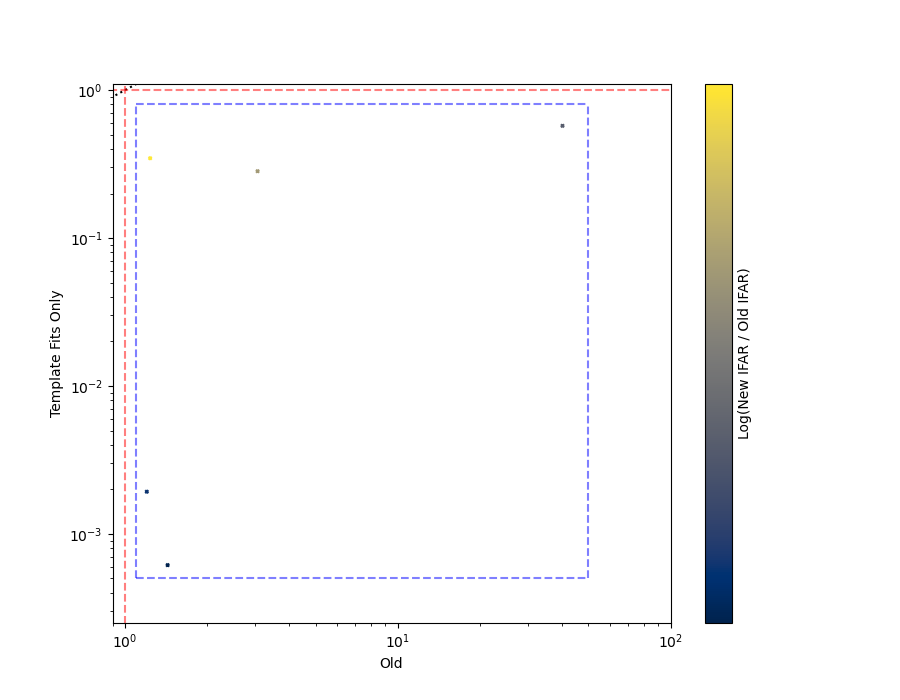
\includegraphics[width=1\textwidth]{images/pycbclive/prev_found_ifar_vs_ifar_region.png}
    \caption{}
    \label{fig:pycbclive-bottom-right-region}
\end{figure}
%
We can look at the numerical values associated with each injection, this is shown in table~\ref{tab:pycbclive-bottom-right-rank-stat}.
%
\begin{table}[ht]
    \centering
    \small
    \setlength{\tabcolsep}{4pt}
    \rowcolors{2}{white}{lightgray}
    \begin{adjustbox}{minipage=\linewidth-0cm, margin=-5cm 0pt 0pt 0cm}
    \begin{tabular}{lccccccccccccc}
        \toprule
        & \multicolumn{4}{c}{\textbf{H1}} & \multicolumn{4}{c}{\textbf{L1}} & \multicolumn{3}{c}{\textbf{New}} & \multicolumn{2}{c}{\textbf{Old}} \\
        \cmidrule(lr){2-5} \cmidrule(lr){6-9} \cmidrule(lr){10-12} \cmidrule(lr){13-14}
        \textbf{Inj Idx} & \textbf{$\rho_{new}$} & \textbf{$\alpha$} & \textbf{$\mu$} & \textbf{ln(r$_n$)} & \textbf{$\rho_{new}$} & \textbf{$\alpha$} & \textbf{$\mu$} & \textbf{ln(r$_n$)} & \textbf{Comb. ln(r$_n$)} & \textbf{ln(r$_s$)} & \textbf{IFAR} & \textbf{ln(r$_s$)} & \textbf{IFAR} \\
        \midrule
        8313 & 5.87 & 2.39 & 15.50 & 5.33 & 12.21 & 3.28 & 19.75 & -16.20 & -14.60 & -15.17 & 0.57 & -15.17 & 40.18 \\
        9120 & 7.83 & 2.89 & 12.69 & -1.69 & 4.89 & 4.07 & 16.49 & 11.25 & 5.83 & -3.10 & 0.00062 & -14.96 & 1.43 \\
        10085 & 5.29 & 2.32 & 10.00 & 8.33 & 6.75 & 1.44 & 18.21 & 2.19 & 6.79 & -0.35 & 0.0019 & -16.15 & 1.20 \\
        10256 & 9.57 & 2.71 & 16.16 & -5.92 & 5.30 & 3.77 & 19.30 & 8.95 & -0.69 & -1.65 & 0.35 & -1.65 & 1.24 \\
        10955 & 8.24 & 2.32 & 10.00 & -2.05 & 9.14 & 1.44 & 18.21 & -1.26 & -7.04 & -8.38 & 0.28 & -8.38 & 3.06 \\
        \bottomrule
    \end{tabular}
    \end{adjustbox}
    \caption{}
    \label{tab:pycbclive-bottom-right-rank-stat}
\end{table}
%
These injections demonstrate a few different cases for injection downranking. Injection $8313$ was found with the same trigger in both searches and while the new statistic's combined noise rate is low it isn't enough to overcome the very low signal rate. The 
$\alpha$ values are low and the $\mu$ values are high indicating poor template fits, and $\rho_{new, H1}$ is below $\rho_{thresh}$ and takes an $\alpha$ of $\alpha_{below} = 6.0$ which (when using equation~\ref{eqn:pycbclive-single-log-noise-rate}) has the function of adding a great amount of log noise rate than if the template's $\alpha$ was used.

Injection $9120$ was found with low SNRs in both detectors with $\rho_{new, L1}$ being below $\rho_{thresh}$ which, as seen by the detector \textbf{ln(r$_n$)} columns, contributes massively to the combined log noise rate. This injection was seen with a different trigger in the new search with a higher signal rate but again, not enough to compensate for the noise rate. This is the same for injections $10085$ and $10256$.

Finally, injection $10955$ was found with the same trigger in both searches and is seen with decent SNR in both detectors but the $\alpha$ values are poor, especially in L1. This produces a high combined log noise rate which the signal rate couldn't overcome. These five injections are problematic, being injections that we have observed with the previous statistic and are now missing but we understand why they have been downranked in each case. Missing these injections is a trade-off with observing so many more newly significant injections.

\subsection{\label{sec:pycbclive-bottom-left}Near-Threshold Injections Still Being Missed}

The final region we are investigating is those injections which were marginally missed near the 1 year threshold when searched for using the old statistic, between an IFAR of 0.1 and 1 years, and then were further downranked by including template fitting in the statistic, these can be seen in the bottom-left quadrant's orange box in figure~\ref{fig:pycbclive-ifar-ifar-fits-only-0s}.  This is an important region because these are the signals which are close to the IFAR threshold and we want to recover these with an improved statistic.

This region contains a large number on injections so we need to look at the broad reasons behind the downranking as opposed to the individual injection reasons. The investigation of this region is where we discovered the impact of the SNR ratio in the noise rate contribution (described in section~\ref{sec:pycbclive-diff-triggers}). Our initial hypothesis was poor fits, similar to the other regions.
%
\begin{figure}
  \centering
  \begin{minipage}[t]{1.0\linewidth}
  
    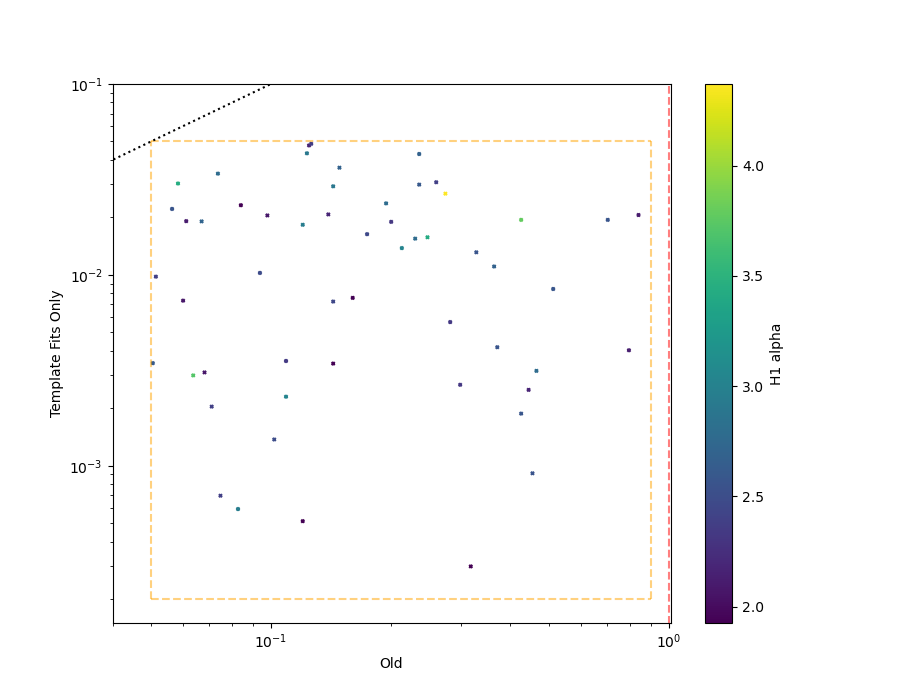
\includegraphics[width=1\textwidth]{images/pycbclive/bl_h1_alpha.png}
    \caption{}
    \label{fig:pycbclive-bottom-left-h1-alpha}
    
    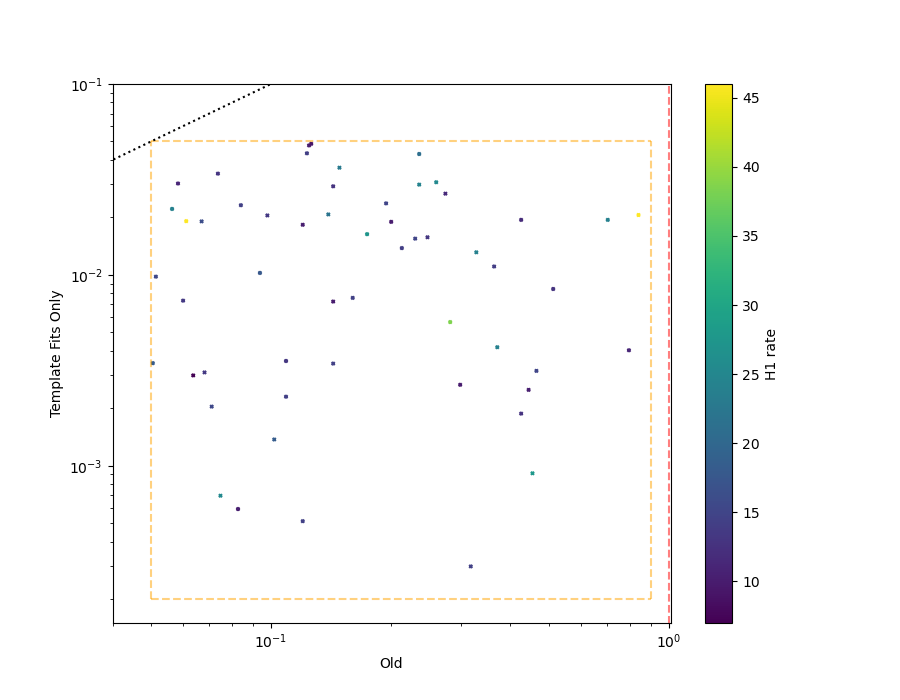
\includegraphics[width=1\textwidth]{images/pycbclive/bl_h1_rate.png}
    \caption{}
    \label{fig:pycbclive-bottom-left-h1-rate}
  
  \end{minipage}
\end{figure}
%
Figures~\ref{fig:pycbclive-bottom-left-h1-alpha} and~\ref{fig:pycbclive-bottom-left-h1-rate} show the IFAR vs IFAR plot for this region with colours representing the H1 $\alpha$ and $\mu$ of each injection. We would hope to see a trend of worse fits the further from the $y=x$ diagonal line we get but the majority of points have low $\alpha$ values with some having high $\alpha$ values. There is a similar story for $\mu$, no clear correlation between $\alpha$ and $\mu$ and injection position in this region.

We can further plot both the single detector H1 log noise rate and the combined log noise rate to see if these are responsible for the downranking, again we would expect to see a higher noise rate the further we are from the diagonal,
%
\begin{figure}
  \centering
  \begin{minipage}[t]{1.0\linewidth}
  
    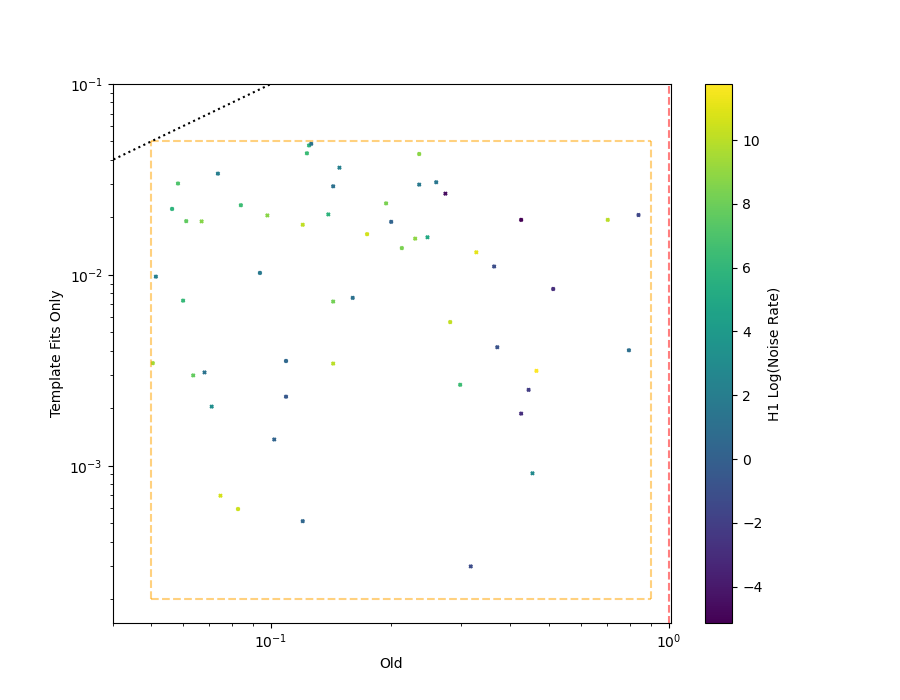
\includegraphics[width=1\textwidth]{images/pycbclive/bl_h1_lognoise.png}
    \caption{}
    \label{fig:pycbclive-bottom-left-h1-log-noise-rate}
  
  % \hspace{0.01\linewidth}
  
    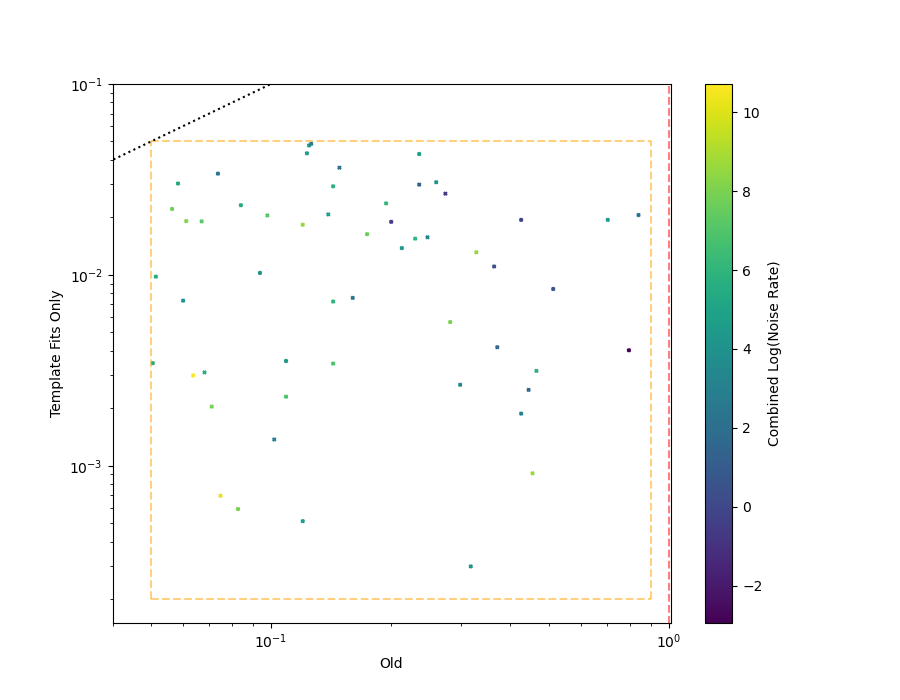
\includegraphics[width=1\textwidth]{images/pycbclive/bl_comb_lognoise.png}
    \caption{}
    \label{fig:pycbclive-bottom-left-comb-log-noise-rate}
  
  \end{minipage}
\end{figure}
%
but from figures~\ref{fig:pycbclive-bottom-left-h1-log-noise-rate} and~\ref{fig:pycbclive-bottom-left-comb-log-noise-rate} we can see that isn't true and in fact some low combined noise rate values for values far from the diagonal. It is at this point we look to the influence of the ranking statistic formulation and more specifically the noise rate contributions, discussed in section~\ref{sec:pycbclive-noise-contrib}. Figure~\ref{fig:pycbclive-bottom-left-snr-ratio} shows the ratio of the two detector $\rho_{new}$ values found by the new statistic (where the ratio is always calculated to be greater than 1)
%
\begin{figure}
  \centering
  \begin{minipage}[t]{1.0\linewidth}
  
    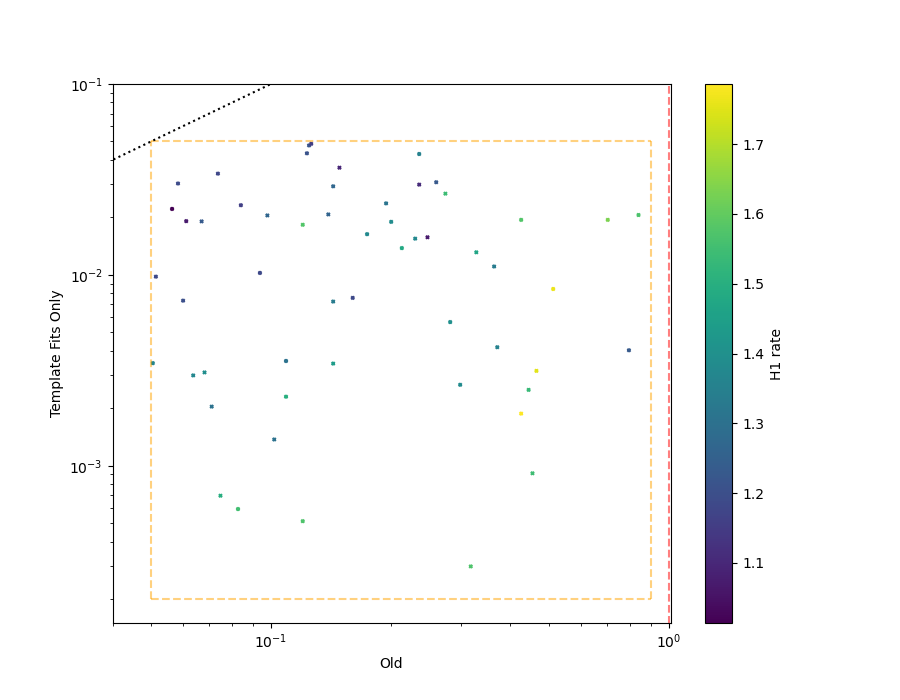
\includegraphics[width=1\textwidth]{images/pycbclive/bl_snr_ratio.png}
    \caption{}
    \label{fig:pycbclive-bottom-left-snr-ratio}
  
  \end{minipage}
\end{figure}
%
This figure tells a large part of the story for this region. There is a visible trend that the injections further from the diagonal have a higher SNR ratio, explaining why they have been downranked to a greater extent that other similar injections. What we are seeing is injections found with a much higher $\rho_{new}$ in one detector when compared to the other, and due to the noise rate contributions described in section~\ref{sec:pycbclive-noise-contrib} and the squared sum of the SNRs being used the difference in SNR value didn't matter as much in the old statistic. In the new statistic however, the contribution from the $\rho_{new}$ is weighted by the template fits parameters $\alpha$ and $\mu$ and simply summed to obtain the combined log noise rate, therefore when one detector has observed a low $\rho_{new}$ it is no longer being compensated for by a large $\rho_{new}$ in the other detector, leading to a dramatic decrease in the significance obtain for these injections.

This is a consequence of the ranking statistic formulation difference between the old statistic and the new statistic and is not concerning, primarily because these injections haven't been seen in the old statistic and still are not seen in the new statistic. We are happy that we understand all three of these regions and the overall sensitivity increase of introducing the new statistic to the live search more than compensates for these injections being downranked.

\subsection{\label{sec:pycbclive-mdc-test}Full Template Bank Test on the Mock Data Challenge Infrastructure}

Finally, we were able to use the PyCBC Live Mock Data Challenge (MDC) testing computational resources to run a full template bank search to test the implementation in an environment that is effectively identical to the actual PyCBC Live search, with the inclusion of the new ranking statistic code. This environment is allocated a number of private nodes equivalent to that of the real PyCBC Live search so we didn't run into the aforementioned memory issues.

We followed the same procedure as done for the offline test, creating template fits across the whole bank for a week of data and then running the search using these template fits on the proceeding weeks. We did not update the fits throughout this test. The purpose of this test was not to test sensitivity improvements, as these have already been tested in offline, it was to test for bugs and if the inclusion of template fits adds any latency to the search. We identified and fixed a number of bugs which were introducing major latency to the search, after fixing there is no latency difference between the current configuration and the new live search configuration.